%%Designed for IEEE Transactions on Vehicular Technology, based on bare_jrnl.tex by Michael Shell.
%%December. 2015
%%Length Requirements: The complete manuscript  should be prepared in final IEEE typesetting with maximum page length limited to 15 pages for a Regular Paper and 5 pages  for a Correspondence. 
%%Contact Info: admin-tvt@ece.ufl.edu
%%Designed by TVT editorial office

\documentclass[journal,10pt]{IEEEtran}

\usepackage{amsmath,scalerel}
\usepackage{enumitem}
\usepackage{enumerate}
\usepackage{tikz}
\usepackage{bbding}
\usepackage{pifont}
\usepackage{wasysym}
\usepackage{amssymb}
\usepackage{enumerate}
\usepackage{pifont}% http://ctan.org/pkg/pifont

\usepackage[utf8]{inputenc}
\usepackage{amsmath,amssymb,amsfonts}
\usepackage{graphicx}
\usepackage{textcomp}
\usepackage{xcolor}
\usepackage{algorithm}
\usepackage{algpseudocode}
\usepackage{multirow}
\usepackage{amsthm}
\usepackage{blindtext}
\usepackage{float}

\newcommand{\var}[1]{\text{\texttt{#1}}}
    \newcommand{\func}[1]{\text{\textsl{#1}}}

    \newcounter{phase}[algorithm]
    \newlength{\phaserulewidth}
    \newcommand{\setphaserulewidth}{\setlength{\phaserulewidth}}
    \newcommand{\Algphase}[1]{%
    \vspace{-1.25ex}
    % Top phase rule
    \Statex\leavevmode\llap{\rule{\dimexpr\labelwidth+\labelsep}{\phaserulewidth}}\rule{\linewidth}{\phaserulewidth}
    \Statex\strut\refstepcounter{phase}\textit{#1}
    % Bottom phase rule
    \vspace{-1.25ex}\Statex\leavevmode\llap{\rule{\dimexpr\labelwidth+\labelsep}{\phaserulewidth}}\rule{\linewidth}{\phaserulewidth}}
    \setphaserulewidth{.7pt}
\makeatother

\begin{document}

\title{Blockchain-based Privacy-Preserving and Sustainable Data Query Service over 5G-VANETs}

\author{Lo-Yao Yeh, Nong-Xiang Shen, Ren-Hung Hwang

\thanks{Lo-Yao Yeh is with the Department of Information Management, National Central University, Taoyuan 320317, Taiwan. (e-mail: yehloyao@ncu.edu.tw)}

\thanks{Nong-Xiang Shen and Ren-Hung Hwang are with the Department of Computer Science Information Engineering, National Chung Cheng University, Chiayi 60102, Taiwan. (e-mail: g08410117@ccu.edu.tw; rhhwang@cs.ccu.edu.tw)
\\ Corresponding Author: Ren-Hung Hwang,  rhhwang@cs.ccu.edu.tw}% <-this % stops a space
}

\markboth{IEEE Transactions on Intelligent Transportation Systems, Manuscript for review}
{Yeh \MakeLowercase{\textit{et al.}}:
Blockchain-based Privacy-Preserving and Sustainable Data Query Service over 5G-VANETs}

\maketitle
% name of $\emph{data\_coin}$

\begin{abstract}
Intelligent Transport Systems (ITSs) play an important role in future smart city design to improve traffic safety and traffic congestion by sharing data collected by vehicles. For sharing the traffic data with other vehicles, the vehicular sensory data are usually uploaded to the cloud server. However, existing data sharing systems for VANETs cannot provide selective data with sufficient privacy protection. Moreover, some schemes also cannot ensure stable data accessibility and the integrity of retrieved data. On the other hand, with the improvements such as lower latency, higher capacity, and increased bandwidth, 5G technology brings more possibilities to future applications. The join of the software-defined networks (SDNs) also offers efficient and effective network management. This paper proposes a primitive vehicular communication system named blockchain-based privacy-preserving and sustainable data query service. The proposed scheme is designed to realize stable data accessibility by leveraging smart contracts and blockchain oracle.
With the help of 5G technology and P2P file-sharing system, InterPlanetary File System (IPFS), the proposed scheme aims to support video downloading files with searchable capability and fairness. An incentive token mechanism is also equipped. The merit of auditability is ensured by Ethereum blockchain platform to support the accountability. Besides, we also evaluate its networking performance via SUMO and NS-3 simulators. Our simulation results show that the request-response delay of BPSDQS is less than existing blockchain-based proxy re-encryption (PRE) scheme. We introduce the on-off model to simulate the online status of the vehicles. Under the condition, the average request-response delay in our scheme can saving up to $98\%$, respectively. 
% , and the smart contract is deployed on Ethereum Remix IDE also demonstrate the practicality of the proposed approach. 
\end{abstract}


\begin{IEEEkeywords}
Vehicular ad-hoc network (VANET), blockchain, software defined network (SDN), proxy re-encryption, InterPlanetary File System (IPFS).
\end{IEEEkeywords}


\IEEEpeerreviewmaketitle



\section{INTRODUCTION}
With the improvement of communication technologies and its software and hardware technologies in recent years, Internet of Things (IoT) devices have been more powerful to assist in decision-making or system control.
In addition, Intelligent Transportation Systems (ITS) is getting more and more attention in the future design of smart cities\cite{Survey on various mechanisms for Secure and Efficient VANET communication}, \cite{Blockchain based intelligent vehicle data sharing framework}.
In order to bring ITS advantages into full play, information sharing takes the critical point.
How to effectively obtain information with security and privacy concerns will be a challenging issue\cite{Security Issues inVehicular Ad-hoc Network(VANET)}\cite{Securing vehicular ad hoc networks}.

Most of the traditional intelligent transportation services are provided by a centralized crowd-server.
This kind of method will greatly rely on network connectivity. Once the traffic is over a certain threshold, it may be unable to provide services, and this centralized system may not afford the huge traffic video file collected by the Vehicular ad hoc networks (VANETs). As a consequence, the crisis of the single point of failure in a centralized system could be serious.
A single point of failure may cause the overall service to fail. At the same time, such a system has the poor ability to withstand malicious attacks. Therefore, current traditional centralized systems may not be suitable for VANETs, and an incentive mechanism is also desired to encourage data owners willing to share their information.
In other words, we will need a decentralized and auditable solution, and that is where blockchain comes into play\cite{Blockchain technology on the way of autonomous vehicles development}. Due to the distributed and shared nature of the blockchain, there is no single point of failure and with transparency merit. In a blockchain platform, each transaction from its source to destination is visible, reducing the opportunities for fraud. As a result, a blockchain-based incentive mechanism is equipped with trustworthiness and fairness, which can also motivate users to share their traffic information.

While a blockchain-based system benefits from its features, it still has some security issues and limitations to be addressed\cite{A survey on the security of blockchain systems}\cite{A blockchain construct for energy trading against sybil attacks}\cite{Regional blockchain for vehicular networks to prevent 51 attacks}. For example, the execution course of smart contracts is exposed to blockchain nodes. Therefore, it is not recommended to calculate the sensitive information on smart contracts. As for limitations, the original design of the blockchain is to record the financial exchange record, which results in small storage size for each block.    

In this paper, a new framework named blockchain-based privacy-preserving and sustainable data query service (BPSDQS) is proposed for ITS deployment. In cooperation with several decentralized technologies such as smart contract, blockchain oracle, and InterPlanetary file system (IPFS), the proposed scheme ensures the features of transparency and reliability. To encourage the contribution of traffic information, a token-based incentive mechanism is also provided. For confidentiality, data owners can encrypt their uploaded video traffic information, and the proposed proxy re-encryption allows the requesting data user to decrypt the re-encrypted file. With the proposed privacy-preserving equality test, a data user can search for the target traffic information without leaking his/her interest keyword. In general, traditional proxy re-encryption approach requires data owners to stay online to provide parameters to re-encrypt the ciphertext. In the proposed scheme, one of the blockchain nodes serving as the blockchain oracle is delegated to take the role of the data owner to get rid of the online restriction. With the help of blockchain oracle, we can provide more stable data accessibility. To overcome the storage limitation, the IPFS can support large amounts of data storage, complementing the blockchain-based system. Furthermore, we take advantage of the 5G technology element, SDN, for efficiently selecting routing paths. 

The contributions of the proposed scheme are summarized as follows: 
\begin{itemize}
  \item [1)]
  the proposed scheme devises a secure proxy-based file encryption to support the sustainable feature and offers privacy-preserving keyword searching merit; 
  \item [2)]
  The proposed platform offers blockahin-based incentive mechanism to meet the requirement of fairness and auditable records; 
  \item [3)]
  The proposed scheme takes advantage of advanced SDN and 5G telecommunication technology that yields efficient response time. 
\end{itemize}

The organization of this paper is as follows. Section II introduces the related works. In section III, we illustrate the preliminaries used in this paper. In sections IV and V, the problem statement and the detailed workflow of our system is described. In section VI, the security of our system will be analyzed. The implementation and performance evaluation of the proposed system is presented in section VII. Finally, the conclusion and future works are discussed in section VIII.

%\hfill August 4, 2015

\section{RELATED WORK}
% 跟現有的相關論文比較
% 幾種可用的論文類型關鍵字:
% vanet 訊息交易
% blockchain
% re-encryption
\subsection{Literature Review}
Due to the features of blockchain, plenty of literature has been proposed to address different issues in VANETs \cite{BECADT}-\cite{Blockchain-enabled security in electric vehicles cloud and edge computing}. 
 \emph{Liu et al.} \cite{BECADT} designed an authentication scheme accompanied by trust management for the proxy vehicles within one RSU to address a cooperative authentication issue on vehicular edge computing. 
 \emph{Xie et al.} \cite{BST} developed a trust management system utilizing blockchain technology over 5G-VANET. With the 5G technology, real-time transmission of high-bandwidth traffic video becomes possible. In their scenario, the video recorded by the vehicles will be tagged and uploaded to the cloud server. The video is encrypted using the owner’s private key such that the video is authenticated and can be viewed by all other users. However, it might lead to a lack of motivation for data sharing.
\emph{Leon et al.} \cite{Secure blockchain-based communication scheme for connected vehicles} proposed a secure communication mechanism to realize secure message exchanges in vehicular platoons. They designed a ring-based signature for platoon joining. However, communication outside the platoon is not considered.
\emph{Li et al.} \cite{Creditcoin: A privacy-preserving blockchain-based incentive announcement network for communications of smart vehicles} proposed a privacy-preserving incentive mechanism based on blockchain technology. It can motivate users to share their traffic information, and the transactions do not leak any information about their sources. Furthermore, the traffic information is not stored on the blockchain but in a cloud server, which, however, may
still encounter the challenges of a centralized server.
\emph{Michelin et al.} \cite{Speedychain: A framework for decoupling data from blockchain for smart cities} designed a blockchain scheme for smart cities. The blockchain is decoupled among different cities. The traffic information is signed by the data owner, and the public key of the data owner needs to be updated in a specific period.
\emph{Chen et al.} \cite{BPREET} proposed a method that combines the proxy re-encryption and equality test to achieve credibility of the test result while maintaining privacy protection. However, proxy re-encryption requires the delegator (data owner) to provide a rekey, which becomes a critical issue needed to be solved. That is, the data owner needs to be always online.
\emph{Liu et al.} \cite{Blockchain-enabled security in electric vehicles cloud and edge computing}
proposed a safety solution based on blockchain protection for electric vehicle energy and data interactions. This scheme uses data coins and energy coins for the interactions between vehicles in order to motivate the vehicles to share data.

Although several works apply blockchain technology in VANETs, the data-sharing scheme in blockchain-based V2V communication has not been considered extensively.
For example, in the above researches, only \cite{BPREET} leveraging proxy re-encryption and equality test to address privacy and data sharing issues. Although the authors of \cite{Blockchain-enabled security in electric vehicles cloud and edge computing} proposed data-sharing via proxy re-encryption, they did not address the cryptography issues. The works \cite{Creditcoin: A privacy-preserving blockchain-based incentive announcement network for communications of smart vehicles}\cite{BPREET}\cite{Blockchain-enabled security in electric vehicles cloud and edge computing} considered the incentive mechanism for transacting traffic information; however, \cite{Creditcoin: A privacy-preserving blockchain-based incentive announcement network for communications of smart vehicles} and \cite{Blockchain-enabled security in electric vehicles cloud and edge computing} introduced blockchain just for the transaction purpose.  As a result, the traffic information is recorded on a centralized server rather than the blockchain, which could be an obstacle to further applications. Our work differs from \cite{BPREET} by proposing solutions that can provide much more stable data accessibility and offer incentive mechanism to encourage the motivation of sharing traffic information. Furthermore, the proposed scheme aims for storing and retrieving video of traffic information by using SDN and 5G technology.

\subsection{Technology Background}
We will briefly describe the technologies introduced in our proposed scheme.

\textbf{Blockchain -}
Blockchain can be regarded as a decentralized database. Its main features include immutability and auditability after uploading the data. A blockchain ledger is jointly maintained by all blockchain nodes.
Therefore, it needs to design a set of methods to maintain the consistency of data. The set of the methods is called the consensus mechanism, such as Proof-of-Work(PoW) and Proof-of-Stack(PoS). In addition, most emerging blockchain technologies now support smart contracts; one of the most famous representatives is Ethereum. A smart contract can be regarded as programable codes that can be executed automatically, and the result states can be uploaded to the blockchain. After meeting certain conditions, the pre-written program in the smart contract can be put into effect. In this way, the blockchain network can provide some services without a centralized cloud server.

\textbf{IPFS -}  
Each block size in a blockchain is limited, and storing a large size of data on the blockchain is infeasible as it will cause a severe impact on the processing time of the consensus mechanism. Hence, a decentralized file system can be introduced to overcome the weaknesses. The proposed scheme would exchange the video messages in our system, so we introduce a P2P distributed file system, InterPlanetary File System(IPFS) technology. All IPFS nodes can obtain files by the IPFS communication protocol and serve as the host to provide part of the file data. The hash value of a file content would be its address, and users can use this address to get the file whenever they want.

\textbf{Searchable encryption -} 
% The encryption of modern cryptography is mainly divided into two ways - symmetric encryption and asymmetric encryption. Symmetric encryption only uses a private key to encrypt and decrypt data, which is faster than asymmetric encryption. Asymmetric encryption uses two keys, a public key and a private key. The two keys are a pair. A private key of the same user corresponds to a public key.
Searchable encryption allows a party to outsource the storage of its data to another party (a server) in a confidential manner while maintaining the ability to search over it selectively. In such a scheme, the data owner encrypts their files and uploads to the cloud server. However, the cloud service provider (CSP) cannot access the content of encrypted files without the data owner's decryption key. Whenever users wish to access their files, they can search over the encrypted files through specific keywords. The searchable encryption generally can be categorized into searchable symmetric-key encryption (SSE) and searchable public-key encryption (SPE). SSE schemes usually have better efficiency, while the overhead of key distribution and management is higher. SPE schemes allow other users to search the encrypted files through the data owner's public key by the keyword, which reduces the cost of key distribution and management but with lower efficiency.

\textbf{Proxy Re-Encryption -}
Proxy re-encryption allows a third-party proxy to convert the ciphertext of the delegator into that of the receiver without revealing the delegator's private key. Therefore, the receiver can decrypt the ciphertext by its private key \cite{Proxy re-encryption with keyword search}. 


\textbf{Blockchain Oracle -}
Based on the shared states, the execution result must be deterministic to maintain consistency among nodes in a blockchain. Therefore, two kinds of operations cannot perform alone. First, there is no intrinsic source of randomness. Second, the extrinsic data can only be updated as the data payload of a transaction. Therefore, the auditable blockchain oracle can fix the gap between the outside world and the blockchain.


\section{PRELIMINARIES}
% 介紹文章需要的基本定義、引理等基礎概念,並進行相關輔助結論的推定工作
% basic knowledge
% security assumption
% Blockchain
% blockchain oracle
% IPFS
% proxy re-encryption
% bilinear pairing
\subsection{Notations}
A summary of notions is listed in TABLE \ref{tab:notation}.

\begin{table}[t!]
\caption{NOTATIONS}
\label{tab:notation}
\centering
\begin{tabular}{ |p{2.3cm}|p{5.5cm}|}
 \hline
 Notations & Descriptions \\
 \hline
 $\lambda$ & security parameter \\
 \hline
 $(q, G_1, G_2, G_T, e)$ & parameters of bilinear pairing \\
 \hline
 $P_{i=1,2}$ & generators of groups $G_{i=1,2}$ \\
 \hline
 $(h_0, H_{i=1,2})$ & hash functions \\
 \hline
 $(pk_i^1, pk_i^2, sk_i)$ & public/secret key tuple of user $u_i$, $pk_i^1, pk_i^2$ are generated from $G_1, G_2$, respectively \\
 \hline
 $(fpk_i^1, fpk_i^2, fsk_i)$ & shared key tuple which are registered by data owner on blockchain oracle, $fpk_i^1, fpk_i^2$ are generated from $G_1, G_2$, respectively  \\
 \hline
  $TK$ & temporary session key that is used to encrypt the message, which will be upload to IPFS \\
 \hline
 $CT_i(KW)$ & ciphertext under $pk_i$ \\
 \hline
 $rk_{oi \to j}$ & re-encryption key generated by the oracle as an identity of user $u_i$ for user $u_j$ \\
 \hline
 $RCT_j(KW)$ & re-encryption ciphertext under $pk_j$ \\
 \hline
 $T_{oi \to j}, T_{j \to oi}$ & authorization trapdoor generated by the blockchain oracle and data user corresponding to $CT_i(KW)$ and $CT_j(KW)$, respectively \\
 \hline
 $||$ & concatenation operation \\
 \hline
 $\oplus$ & Bitwise xor operation \\
 \hline
\end{tabular}
\end{table}

\subsection{Bilinear Pairing}
Let $G_1, G_2, G_T$ be multiplicative cyclic groups with prime order q. Let $P_i$ be the generator of group $G_i$, where $i$=1, 2. Let $e$ be a bilinear map $e : G_1 \times G_2 \to G_T$ with the following properties:
\begin{itemize}
  \item \textbf{Bilinearity:}
  For all $u \in G_1, v \in G_2$, and any $a,b \in Z_q^*$, equation $e(u^a,v^b) = e(u,v)^{ab}$ holds.
  \item \textbf{Non-degeneracy:}
  $e(u,v) \neq 1_{G_T}$
  \item \textbf{Computability:}
  For any $u \in G_1$ and $v \in G_2$, there exist a polynomial complexity algorithm to  compute $e(u,v) \in G_T$
  
\end{itemize}

\subsection{Hard Problem Assumption} 
The security of our scheme is based on following hard problem:
\subsubsection{Computional Diffie-Hellman (CDH) assumption \cite{Introduction to Modern Cryptography}}
 Let $G_1$ be a cyclic group of order $q$, and $P$ is the generator of $G_1$. Given $(P,xP,yP) \in G_1$ with random number %variables 
 $x,y \in Z_q^*$. Let A be the algorithm that returns an element of G. The advantage for a polynomial-time bounded adversary using algorithm A to computes $xyP \in G_1$ is defined as

\begin{center}
$Adv_{G,P}^{CDH}(A) = Pr[A(P,xP,yP) = xyP] \leq \varepsilon$
\end{center}

\subsubsection{Decisional Bilinear Diffie-Hellman (DBDH) assumption \cite{New directions in cryptography}}
Let $(G_1, G_2, G_T)$ be three groups with the same order $q$. Let e be the bilinear pairing $e(P_1, P_2) \in G_T$. Given $(P_1,xP_1,yP_2,zP_1,e(P_1,P_2)^{xyz})$ with random $x,y,z \in Z_q^*$ and a random tuple $(P,xP_1,yP_2,zP_1,Z\xleftarrow[]{rand}G_T)$ with random $x,y,z \in Z_q^*$. The advantage for a polynomial-time bounded adversary using algorithm A to determine that whether $Z=e(P_1,P_2)^{xyz}$ is defined as

\begin{center}
$Adv_{G,P}^{DBDH}(A) = |Pr[A(P,xP_1,yP_2,zP_1,e(P_1,P_2)^{xyz})]-Pr[A(P,xP_1,yP_2,zP_1,Z]| \leq \varepsilon$
\end{center}

We said that both the CDH and the DBDH assumptions are hold if %the advantage 
$Adv_{G,P}^{CDH}(A)$ and $Adv_{G,P}^{DBDH}(A)$ are negligible. These problems are nearly impossible for a polynomial-time bounded adversary to solve, that is, $\varepsilon$ is negligible.


\section{PROBLEM STATEMENT}
% system model
% security assumption
% design goals
In this section, we formulate the system model and design goals of our scheme.
\subsection{System Model} 
In a data-sharing system, commuters with common interests can share data with others in order to promote transport efficiency and safety. We consider a complete data sharing scheme in our system, where authorized data user and data owner need to upload their encrypted messages(e.g., traffic information in the text or video format) and keywords(e.g., tags of traffic information) to the IPFS and blockchain. Data users can search for the target traffic information by the tags of the encrypted messages. Fig. \ref{fig:work_flow} shows the scenario of our scheme. We abstract five modules in our scheme as special entities, including trust authority, data owner, data user, blockchain oracle, and IPFS.

\subsubsection{\textbf{Trusted Authority}}
The trusted authority (TA) is an off-chain trusted third party to generate system parameters, distribute keys, and deploy smart contracts.
% \subsubsection{\textbf{RSU}}
% A Roadside Unit (RSU) is a wireless access point that is mounted aside a road. In our scenario, a RSU is controlled by SDN controllers, some RSU will work as a blockchain node or even a role of blockchain oracle.

\subsubsection{\textbf{Data owners}}
Data owners are the commuters who publish the encrypted keywords to the smart contract and the encrypted message (e.g., traffic information in video form) to IPFS. Before uploading these messages to the proposed platform, the data owners need to register to the TA and blockchain oracle to get their key pairs.
\subsubsection{\textbf{Data users}}
Data users are the consumers of the messages (e.g., video or road conditions). They can search the target messages by using encrypted keywords.
\subsubsection{\textbf{Blockchain oracle}}
In our scenario, the blockchain oracle is introduced to delegate the data owner, who may not always be online. That is, the commuters who are data providers on the blockchain need to register to the blockchain oracle to get their key pair. In this way, the blockchain oracle can act as the data owner to provide necessary security parameters to the smart contract for sharing messages to data users.
\subsubsection{\textbf{IPFS}}
In our scheme, IPFS is responsible for storing large files such as video records and messages of traffic conditions. 

\begin{figure*}[h!]
    \centering
    \resizebox{\textwidth}{!}{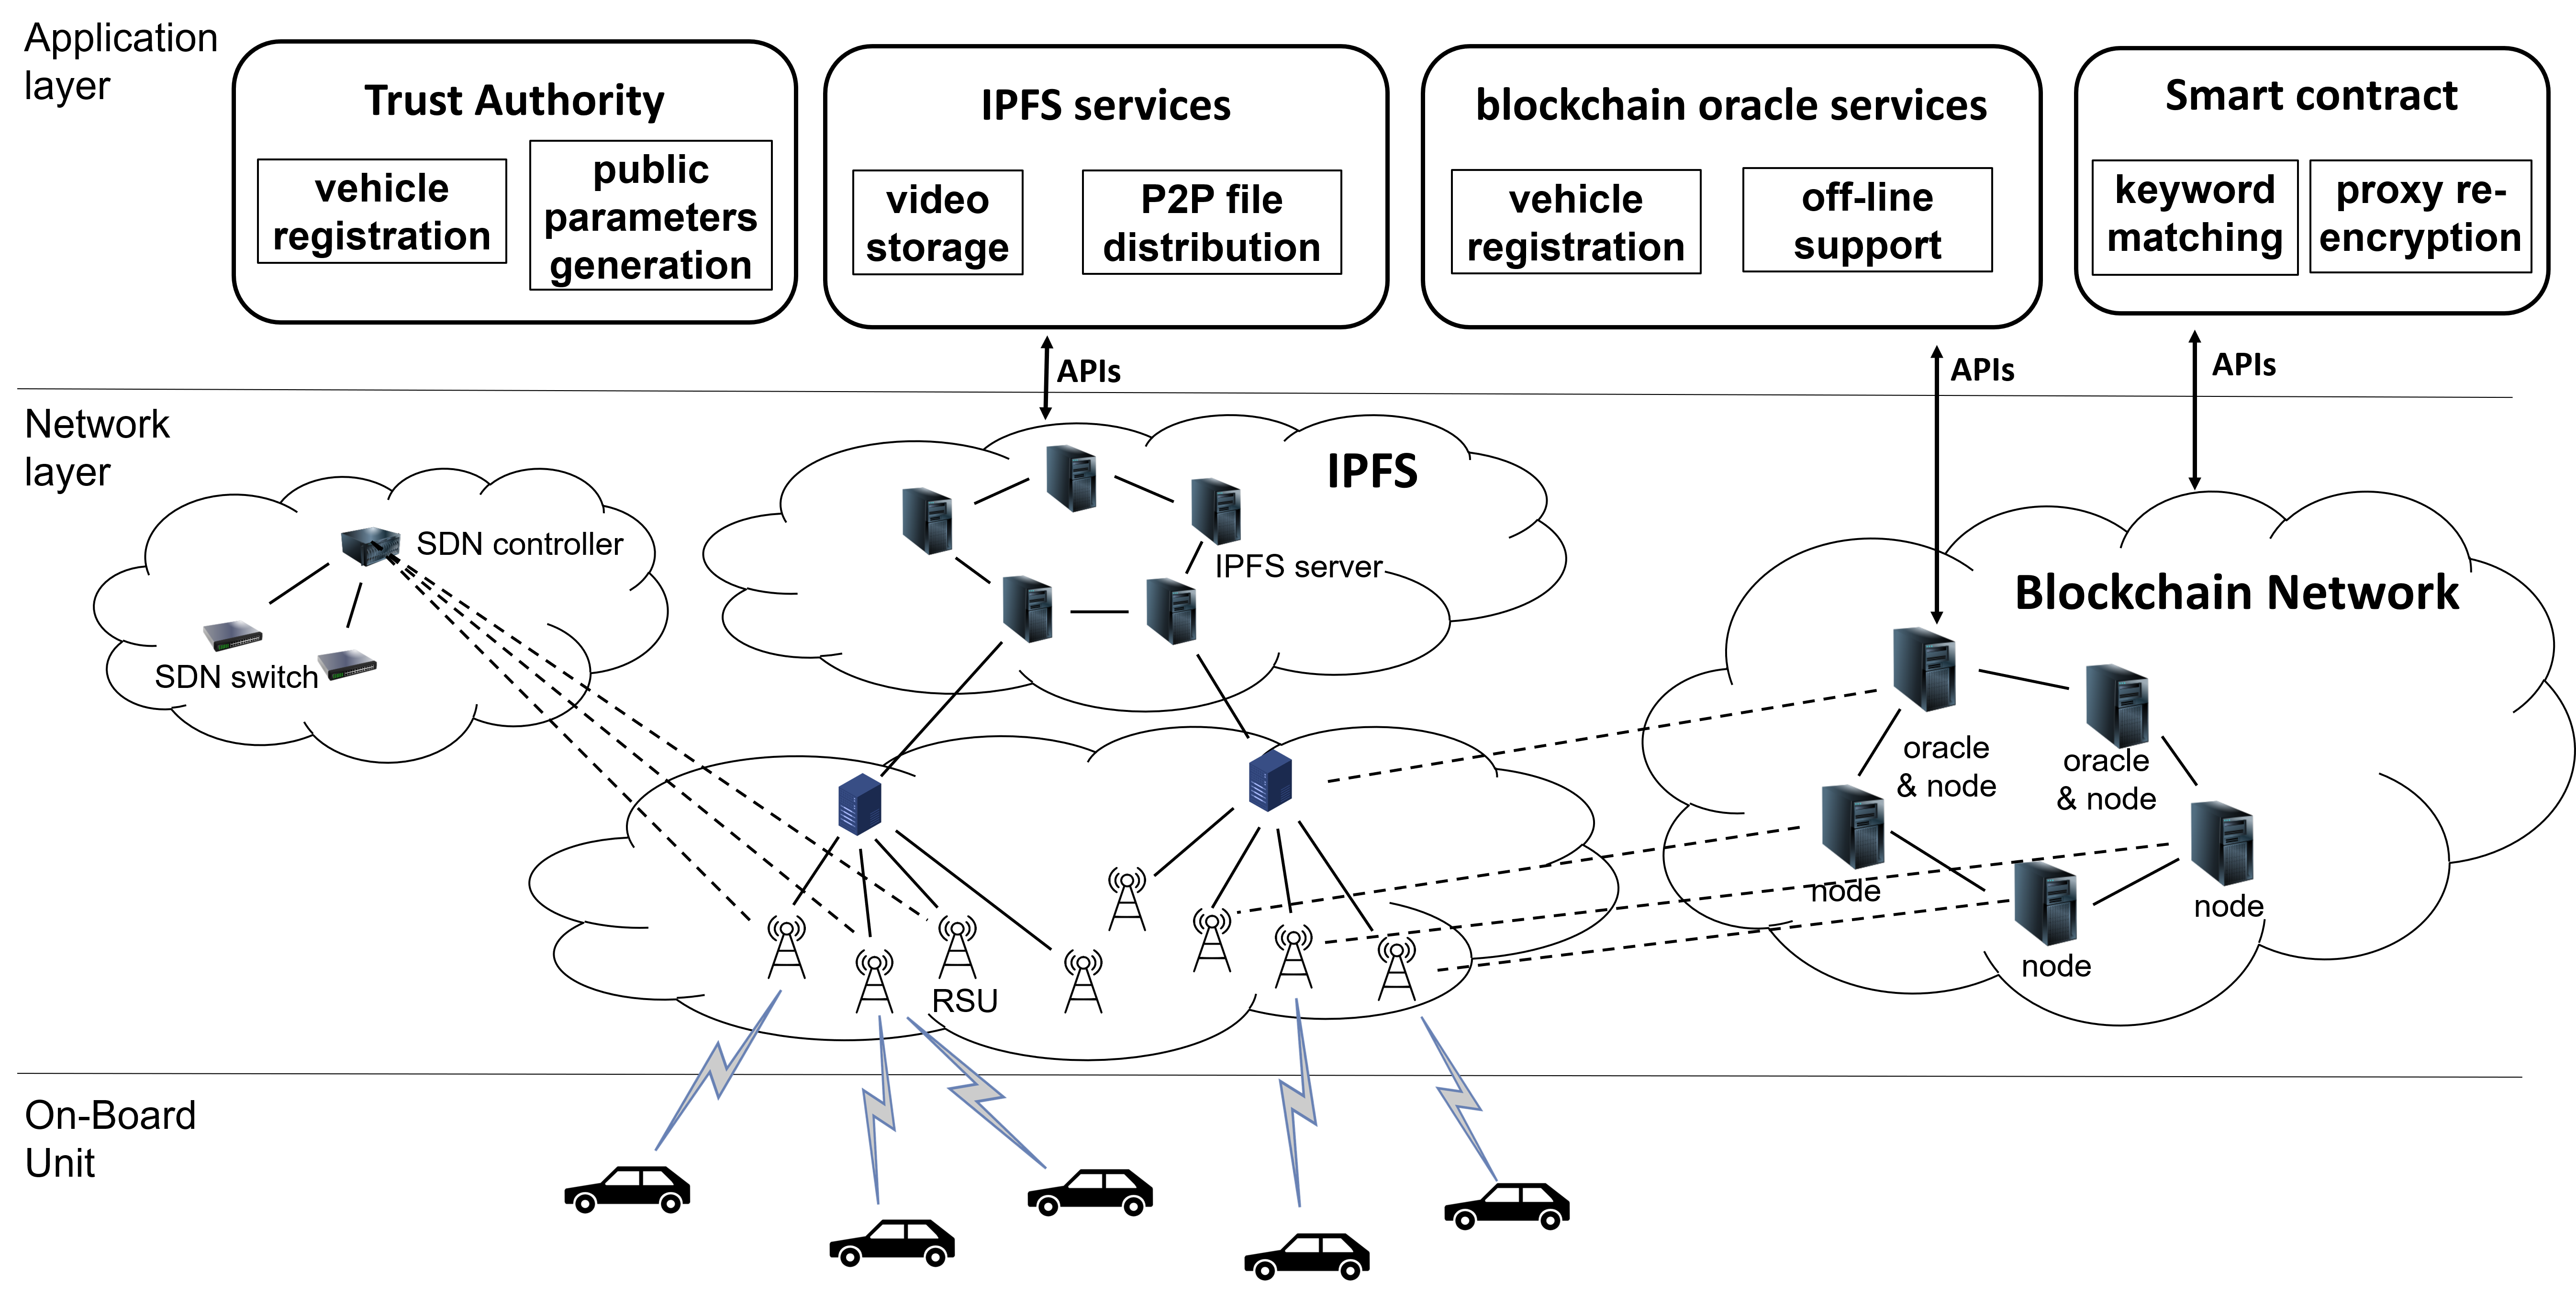
\includegraphics{picture/arch5.png}}
    \caption{System Architecture}
    \label{fig:architecture}
\end{figure*}

\subsection{Threat Models}
The smart contracts are public and transparent. The adversary will come from outside the system and try to get private messages such as keywords and traffic information content (e.g., video records). Also, they will try to access secret parameters via ciphertexts, trapdoors, and rekeys. The adversary is assumed to be a polynomial-time entity.

\subsection{Design Goals} 
\begin{itemize}
  \item \textbf{Confidentiality:}
  Confidentiality means that both of data user and data owner's message (keyword) should be protected from the adversary.
  \item \textbf{Searchability and Privacy:}
  For searchability, the data users can search for the wanted data by the keyword and equality test algorithm. In terms of privacy, the searching keyword issued by the data user should not be leakage to anyone.
  \item \textbf{Stable Data Accessibility:}
  Stable data accessibility requires that whenever the data users query for the data, the system will always be able to provide data accessibility. Since data owners are not always online, the proposed scheme arranges the blockchain oracle as the role of proxy agent for the data owner.
  \item \textbf{Decentralization and Transparency:}
  The decentralization and transparency mean that the whole system does not rely on centralized servers. Instead, multiple nodes take part in maintaining the ledger and performing the program code of the smart contract, which also provides the merit of auditability.
\end{itemize}

\subsection{Architecture} 
% 描述有關的系統架構 
% (葉羅堯註記)本段落應該要移到前面System model 搭配今天說的那個三層的圖,所以應該會需要重寫
In our system architecture (see Fig. \ref{fig:architecture}), we introduce Software Defined Networks (SDN) into the data plane of the 5G network. The SDN technology is applied in the network in order to build up a powerful and effective VANET. Specifically, SDN is introduced to reduce upload and download delay in the 5G network by better routing control.

\subsection{System overview} 
As shown in Fig. \ref{fig:work_flow}, if a data owner has some video records of traffic information and wishes to publish this information in to the system, the content and the keyword about the records will be encrypted and sent to the IPFS and smart contract, respectively. Once a data user requests for these video records, the data user should select the suitable keyword and perform the interest matching as the filter to pick up the desired records. The smart contracts will verify  whether the data owner's keyword is the same as the data user's. If yes, the blockchain oracle and smart contract will cooperate to re-encrypt the ciphertext. Next, if the data user can offer enough $\emph{data\_coin}$ for purchasing the video record, then the data user can retrieve the corresponding security parameters. In the end, the data user can  obtain the ciphertext from the IPFS and decrypt it. Furthermore, the data owner and the blockchain oracle can earn the deserved $\emph{data\_coin}$.  

\begin{figure}[h]
    \centering
    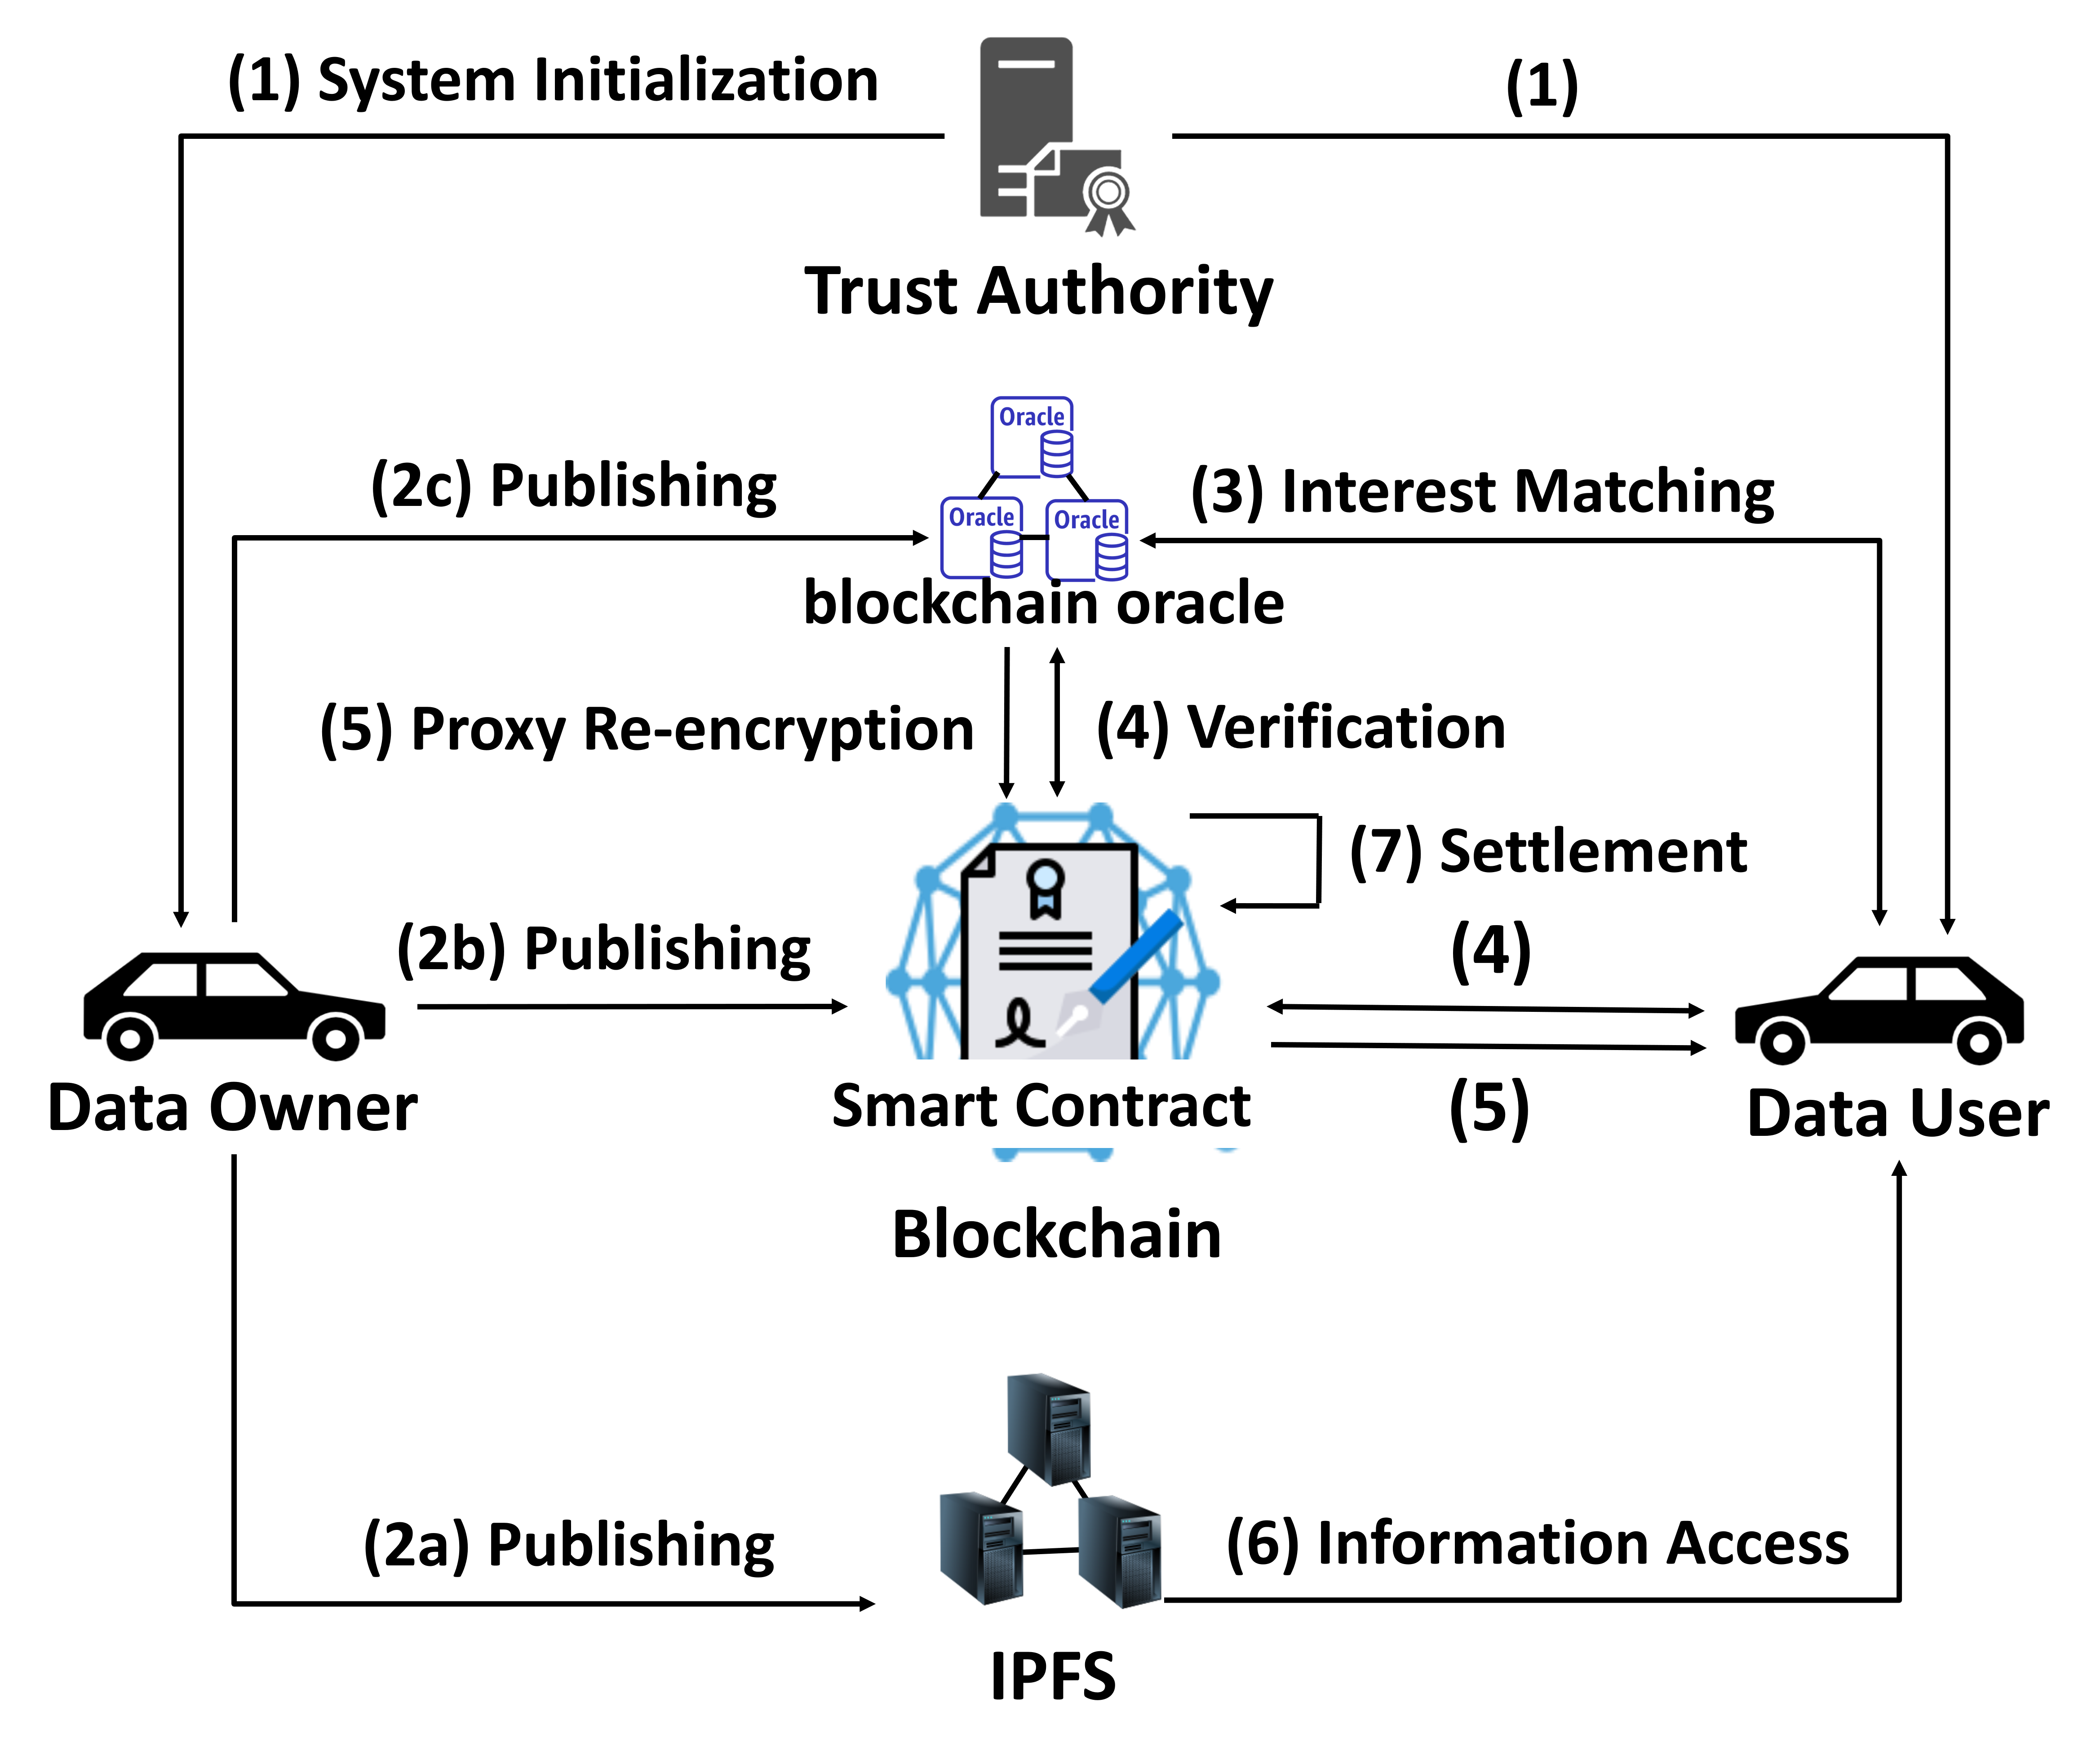
\includegraphics[width=260pt]{picture/flow2.png}
    \caption{Work flow}
    \label{fig:work_flow}
\end{figure}

\section{CONSTRUCTION}

\subsection{System Operations}
In this paper, a new adaptive proxy encryption is proposed and the operations related to constructing the proposed scheme are as follows:

\begin{itemize}
    \item $ \boldsymbol{Setup}(1^\lambda) \to pp $: 
    The algorithm is executed by trust authority to do the system initialization. It takes security parameter $1^\lambda$ as input 
    and selects bilinear group ${G_1, G_2, G_T}$ with the same prime order \emph{q}. 
    The bilinear pairing operation is ${e:G_1\times G_2 \to G_T}$.
    It will select three secure hash functions $h_0:\{0,1\}^* \to Z_q^*, H_1: G_1 \to \{0,1\}^{4\lambda}$ and $H_2:G_2 \times G_1 \times G_1 \to Z_q^*$.
    Finally, it publishes the parameter $pp = \{G_1, G_2, G_T, q, P_1, P_2, e, h_0, H_1, H_2\}$.
    
    \item $ \boldsymbol{KeyGen}(pp) \to (sk_i, fsk_i, pk_i^1, pk_i^2, fpk_i^1, fpk_i^2) $: The algorithm is used to generate the secret/public key pairs. A user $u_i$ will randomly select two numbers as secret key:
    
    (1) $sk_i = a_i \xleftarrow{R} Z_q^*$ in the main system
    
    (2) $fsk_{oi} = b_i \xleftarrow{R} Z_q^*$ shared with the blockchain oracle system
    
    The public keys for $u_i$ will be generated: 
    
    (3) $pk_i^1 = sk_i \cdot P_1, $
    
    (4) $pk_i^2 = sk_i \cdot P_2, $
    
    (5) $fpk_{oi}^1 = fsk_{oi} \cdot P_1,$
    
    (6) $fpk_{oi}^2 = fsk_{oi} \cdot P_2$. 
    
    The tuple $(sk_i, pk_i^1, pk_i^2)$ is used in the main system, and the tuple $(fsk_{oi}, fpk_{oi}^1, fpk_{oi}^2)$ is used in the blockchain oracle system.
    
\end{itemize}

\begin{itemize}
    \item $ \boldsymbol{Encrypt}(pp, sk_i, fsk_{oi}, KW_i, TK) \to CT_i(KW) $: The algorithm is used to calculate ciphertext. It takes public parameter $pp$, the private key of the user $u_i$, the public key of the user $u_i$, which is registered on the blockchain oracle, the keyword message $KW$, and the temporary session key $TK$ as its input. Each part in $CT_i(KW)$ is computed as follows: 
    
    (1) $C_{i1} = r_{i1} \cdot r_{i2} \cdot P_2$
    
    (2) $C_{i2} = r_{i1} \cdot r_{i2} \cdot h_0(KW_i) \cdot P_1 + r_{i3} \cdot P_1$ 
    
    (3) $C_{i3} = (KW_i||TK||r_{i1}||r_{i3}) \oplus H_1(r_{i2} \cdot fsk_{oi} \cdot sk_i \cdot P_1)$
    
    (4) $V_{KW} = H_2(C_{i1}||C_{i2}||(r_{i2} \cdot P_1))$
    
    (5) $D_{KW} = r_{i2}-V_{KW} \cdot fsk_{oi}$
    
    (6) $CT_i(KW) = \{C_{i_1}, C_{i_2}, C_{i_3}, V_{KW}, D_{KW}\}$ will be returned.
\end{itemize}

\begin{itemize}
    \item $ \boldsymbol{Decrypt}(pp, CT_i(KW), sk_{i}, fsk_{oi}) \to \{(KW||TK||r_{i1}||r_{i3}), r_{i2}\} $: This algorithm is used to decrypt the ciphertext, which is generated by the decrypter. It takes public parameter $pp$, Ciphertext $CT_i(KW)$, private key $sk_{i}$, and shared key $fsk_{oi}$ as input. Each part of the result is computed as follows: 
    
    (1) $r_{i2} = D_{KW} + V_{KW} \cdot fsk_{oi}$
    
    (2) $(KW||TK||r_{i1}||r_{i3}) = C_{i3} \oplus H_1(r_{i2} \cdot fsk_{oi} \cdot sk_i \cdot P_1)$
    
    The result could be verified by checking if: 
    
    (3) $C_{i1} = r_{i1} \cdot r_{i2} \cdot P_2$
    
    and 
    
    (4) $C_{i2} = (r_{i1} \cdot h_0(KW) \cdot r_{i2} \cdot P_1) + r_{i3} \cdot P_1$
    
    
    \item $ \boldsymbol{Trapdoor}(pp, pk_j, fsk_{oi}/sk_j, CT_i(KW)) \to T_{oi \to j} $: The algorithm is executed by the blockchain oracle or data user to generate the trapdoor, which will be an input for $\boldsymbol{Test}$ to do the equality test. It takes public parameter $pp$, the public key $pk_j$ of data user $u_j$, shared key $fsk_{oi}$ or private key $sk_j$ , and the Ciphertext $CT_i(KW)$ encrypted by data user $u_i$ as input.
    
    (1) Recover $r_{i1}, r_{i3}$ by decrypt $CT_i(KW)$ and $r_{i2} = D_{KW} + V_{KW} \cdot fsk_{oi}$. 
    
    (2) The trapdoor $T_{oi \to j} = r_{i1} \cdot r_{i2} \cdot fsk_{oi} \cdot pk_j - r_{i3} \cdot P_1$.
    
\end{itemize}



\begin{itemize}
    \item $ \boldsymbol{Rekey}(pp, pk_i, fsk_{oi}, CT_i(KW), pk_j) \to rk_{oi \to j}$: The algorithm will generate the rekey, which will be an input in the $ReEncrypt$ algorithm. It takes public parameter $pp$, the public key $pk_j$ of data user $u_j$, public key $pk_i$, shared key $fsk_{oi}$ used in blockchain oracle system, and the ciphertext $CT_i(KW)$ from the data owner as input.
    The detail is described as follows:
    
    (1) $r_{i2} = D_{KW} + V_{KW} \cdot fsk_{oi}$
    
    (2) $rk_{oi \to j} = H_1(r_{i2} \cdot fsk_{oi} \cdot pk_i) \oplus H_1(r_{i2} \cdot pk_j)$
    
    (3) $rk_{oi \to j}$ will be returned.
    
    \item $ \boldsymbol{ReEncrypt}(CT_i(KW), rk_{oi \to j}) \to RCT_j(KW)$:
    The ciphertext $CT_i(KW)$ will be re-enctrypted by the rekey $rk_{oi \to j}$ generated by the algorithm $\boldsymbol{ReKey}$.
    The detail is described as follows:
    
    (1) $C_{j3} = C_{i3} \oplus rk_{oi \to j} = (KW||TK||r_{i1}||r_{i3}) \oplus  H_1(r_{i2} \cdot fsk_{oi} \cdot sk_i \cdot P_1) \oplus H_1(r_{i2} \cdot fsk_{oi} \cdot pk_i) \oplus H_1(r_{i2} \cdot pk_j)  = (KW||TK||r_{i1}||r_{i3}) \oplus H_1(r_{i2} \cdot pk_j)$
    
    (2) $C_{j1} = C_{i1}, C_{j2} = C_{i2}$
    
\end{itemize}

\begin{itemize}
    \item $ \boldsymbol{ReDecrypt}(pp, RCT_j(KW), sk_{j}, fpk_{oi}^1) \to \{(KW||TK||r_{i1}||r_{i3})\} $: The algorithm is executed by the user to decrypt the ciphertext, which is re-encrypted by smart contract.
    It takes public parameter $pp$, Ciphertext $RCT_j(KW)$, private key $sk_{j}$, and public key $fpk_{oi}^1$ as input. Each part of the result is computed as follows: 
    
    (1) $R = D_{KW} \cdot P_1 + V_{KW} \cdot fpk_{oi}^1$
    
    $= (r_{i2} - V_{KW} \cdot fsk_{oi}) \cdot P_1 + V_{KW} \cdot fsk_{oi} \cdot P_1$
    
    $= r_{i2} \cdot P_1$
    
    (2) $r_{i2} \cdot P_2  = D_{KW} \cdot P_2 + V_{KW} \cdot fpk_{oi}^2$
    
    (3) $(KW||TK||r_{i1}||r_{i3}) = C_{j3} \oplus H_1(sk_j \cdot R)$
    
    The result could be verified by: 
    
    (4) $C_{j1} = r_{i1} \cdot r_{i2} \cdot P_2$
    
    (5) $C_{j2} = (r_{i1} \cdot h_0(KW) \cdot R) + r_{i3} \cdot P_1$
\end{itemize}
\begin{itemize}
    \item $ \boldsymbol{Test}(pp, C_{i1}, C_{i2}, T_{oi \to j}, C_{j1}, C_{j2}, T_{j \to oi}) \to \{True/False\} $: The algorithm will be executed by the blockchain oracle and the data user to perform the self-test of equality test. Also, it will be executed by smart contract as a verification evidence.
    For the convenience of description, the data user is denoted as $u_j$. The $\boldsymbol{Test}$ algorithm takes the public parameters $pp$, $C_{i1}$, and $C_{i2}$ from $CT_i(KW)$, trapdoor $T_{oi \to j}$ generated by the oracle as the proxy of data owner $u_i$, $C_{j1}$, and $C_{j2}$ from $CT_j(KW)$, and trapdoor $T_{j \to oi}$ generated by the user $u_j$.
    The algorithm goes as follows:
    
    (1) $TC_i = C_{i2} + T_{oi \to j} = r_{i1} \cdot r_{i2} \cdot h_0(KW_i) \cdot P_1 + r_{i3} \cdot P_1 + r_{i1} \cdot r_{i2} \cdot fsk_{oi} \cdot pk_j - r_{i3} \cdot P_1$
    
    (2) $TC_j = C_{j2} + T_{j \to oi} = r_{j1} \cdot r_{j2} \cdot h_0(KW_j) \cdot P_1 + r_{j3} \cdot P_1 + r_{j1} \cdot r_{j2} \cdot sk_{j} \cdot fpk_{oi} - r_{j3} \cdot P_1$
    
    (3) Test if $e(TC_j, C_{i1})$ is equal to $e(TC_i, C_{j1})$. If $KW_i$ equals to $KW_j$, it will return true, otherwise it will return false.
    
\end{itemize}

\subsection{Work Flow}
Fig. \ref{fig:work_flow} shows the overall interactions of the BPSDQS system. 
The details of each stage are described as follows:

\subsubsection{\textbf{System Initialization}}
The TA first runs the \boldsymbol{Setup} algorithm to initialize the system parameters. Then, all users will execute the \boldsymbol{KeyGen} algorithm to generate the corresponding public/private key pairs for the main system and shared key for the blockchain oracle. TA will publish the public parameter $pp = \{G_1, G_2, G_T, q, P_1, P_2, e, h_0, H_1, H_2\} $. The smart contract will be deployed to generate our incentive coin named $\emph{data\_coin}$. Each user will be granted a certain amount of $\emph{data\_coin}$ in his/her blockchain address.

\subsubsection{\textbf{Traffic Information Publishing}}
In this stage, data owner $u_i$ may generate ciphertext of traffic information(e.g., ciphertext of traffic conditions and video records) and the relevant encrypted keyword messages. Then, these messages will be published to the smart contract and the IPFS. The detail is described as follows:

\begin{enumerate}[a.]
    
    \item 
    The data owner $u_i$ will encrypt the video record of road conditions using the temporary session key $TK$ and upload it to the IPFS. In return, the data owner $u_i$ will get the download URL on the IPFS.
    
    \item 
    The data owner $u_i$ will generate  $CT_i(KW) = \{C_{i_1}, C_{i_2}, C_{i_3}, V_{KW}, D_{KW}\}$ by the \blodsymbol{Encrypt} function. Then, the data owner $u_i$ sends a transaction to the smart contract with the payload $<CT_i(KW), URL>$. After uploading the encrypted traffic information, the data owner will get some $\emph{data\_coin}$ as an incentive from the blockchain system. The smart contract will specify the price of $\emph{data\_coin}$ for the specific amount of traffic information.
    
    \item 
    The data owner $u_i$ has several shared key $fsk_i$ with blockchain oracle. The data owner should notify the blockchain oracle which index of the shared key that the data owner wants to use.
    %The Data owner should notice blockchain oracle that which index of shared key that data owner want to use.
    
\end{enumerate}

\subsubsection{\textbf{Interest Matching}}
Once a data user $u_j$ wants to get the messages she is interested, she will compute the $CT_j(KW)$, which includes the keyword message $KW$, by leveraging the \boldsymbol{Encrypt} algorithm. Then, the keyword message will be sent to the blockchain oracle to search for the correct information. After receiving the $CT_j(KW)$, the blockchain oracle will compare to the target messages by performing the $Trapdoor$ algorithm to generate trapdoors as inputs in the $Test$ algorithm to do the equality test. Once the blockchain oracle has collected those messages which can be matched, these candidate messages $CT_{1..k}(KW)$, where $k$ is the number of match messages, will be sent back to the data user $u_j$. Then, the data user $u_j$ will send the index $index_{CT_i}$, which denotes the chosen index of $CT_i(KW)$, to the blockchain oracle.

\subsubsection{\textbf{Verification}}
After receiving $index_{CT_i}$ from the data user $u_j$, the blockchain oracle will calculate and send $T_{oi \to j}$ to the smart contract. On the other hand, the data user $u_j$ will also send $CT_j(KW_j)$, $T_{j \to oi}$, and enough $\emph{data\_coin}$ to the same smart contract. After receiving the necessary messages, the smart contract will perform the $\boldsymbol{Test}$ algorithm in order to verify whether the $KW_i$ and $KW_j$ are matched. The smart contract will fill the result in its table. If the result is negative, the smart contract will return the appropriate $\emph{data\_coin}$ back to the data user's address.

\subsubsection{\textbf{Proxy Re-Encryption}}
The blockchain oracle will listen to the result on the smart contract by the events. If the verification result on the smart contract is true and the payment is ready, the blockchain oracle will perform the $\boldsymbol{Rekey}$ algorithm to produce the rekey $rk_{oi \to j}$. The $rk_{oi \to j}$ will be sent to the smart contract for the data user.

\subsubsection{\textbf{Access to Information}}

Once obtaining the rekey $rk_{oi \to j}$, the data user $u_j$ can run $\boldsymbol{ReEncrypt}$ algorithm to generate the re-encrypted ciphertext. Then, the data user can use its private key $sk_j$ to perform the $\boldsymbol{ReDecrypt}$ algorithm to get the temporary key $TK$. After downloading the encrypted video from the IPFS, the data user can decrypt the video records by the temporary session key $TK$.

\subsubsection{\textbf{Settlement}}
% 清算
If the above operations are finished, the data owner and blockchain oracle will get their deserved $\emph{data\_coin}$ from the data user by the smart contract. As a result, the data provider and the helper, i.e., the blockchain oracle, are encouraged to contribute more data and computing resources to facilitate the traffic information sharing.

\section{SECURITY ANALYSIS}

In this section, we analyze the security properties as follows.

\subsection{Confidentiality}
% ciphertext

\textbf{Lemma 1.} 
The $Encryption$ algorithm used in BPSDQS is confidential if and only if 
the computational Diffie-Hellman assumption is hold and the hash functions are collision-resistant.

\textbf{Proof.}
The challenger C generates the ciphertext $CT_i(KW)=\{C_{i_1}=r_{i1} \cdot r_{i2} \cdot P_2, C_{i_2}=r_{i1} \cdot r_{i2} \cdot h_0(KW) \cdot P_1 + r_{i3} \cdot P_1, C_{i_3}=(KW||TK||r_{i1}||r_{i3}) \oplus H_1(r_{i2} \cdot fsk_{oi} \cdot sk_i \cdot P_1), V_{KW}=H_2(C_{i1}||C_{i2}||(r_{i2} \cdot P_1)), D_{KW}=r_{i2}-V_{KW} \cdot fsk_{oi}\}$, where $r_{i1},r_{i2},r_{i3}$ are randomly selected from $Z_q^*$. 
As we can see in the $CT_i(KW)$, $C_{i_3}$ is calculated by $C_{i_3}=(KW||TK||r_{i1}||r_{i3}) \oplus H_1(r_{i2} \cdot fsk_{oi} \cdot sk_i \cdot P_1)$. From the view of the adversary, the tuple $(r_{i2} \cdot P_1 , fsk_{oi}  \cdot P_1, sk_i \cdot P_1 , r_{i2} \cdot fsk_{oi} \cdot sk_i \cdot P_1)$ forms a CDH problem since that $(r_{i2}, fsk_{oi}, sk_i)$ are randomly selected and unknown. That is, the adversary cannot determine the relationship between message $(KW||TK||r_{i1}||r_{i3})$ and $H_1(r_{i2} \cdot fsk_{oi} \cdot sk_i \cdot P_1)$ based on the knowledge $(P_1, r_{i2} \cdot P_1,  fsk_{oi}  \cdot P_1, sk_i \cdot P_1)$. The advantage for the adversary to reveal the information about plaintext by the ciphertext is negligible.

\subsection{Searchability and Privacy}
% trapdoor 

The correctness of searchability is ensured as follows:

\begin{center}
$e(TC_j, C_{i1}) = e(r_{j1} \cdot r_{j2} \cdot h_0(KW_j) \cdot P_1 + r_{j1} \cdot r_{j2} \cdot sk_j \cdot fpk_{oi}, r_{i1} \cdot r_{i2} \cdot P_2)$
    
$= e(r_{j1} \cdot r_{j2} \cdot h_0(KW_j) \cdot P_1 + r_{j1} \cdot r_{j2} \cdot sk_j \cdot fsk_{oi} \cdot P_1, r_{i1} \cdot r_{i2} \cdot P_2)$
    
$= e((h_0(KW_j) + sk_j \cdot fsk_{oi}) \cdot r_{j1} \cdot r_{j2} \cdot P_1, r_{i1} \cdot r_{i2} \cdot P_2)$,
\end{center}
and
\begin{center}
$e(TC_i, C_{j1}) = e(r_{i1} \cdot r_{i2} \cdot h_0(KW_i) \cdot P_1 + r_{i1} \cdot r_{i2} \cdot fsk_{oi} \cdot pk_j, r_{j1} \cdot r_{j2} \cdot P_2)$

$= e((h_0(KW_i) + sk_j \cdot fsk_{oi}) \cdot r_{i1} \cdot r_{i2} \cdot P_1, r_{j1} \cdot r_{j2} \cdot P_2)$,
\end{center}
thus, according to the bilinear pairing operation, it can be rewritten as
\begin{center}
$e(TC_i, C_{j1})= e((h_0(KW_i) + fsk_{oi} \cdot sk_j) \cdot r_{j1} \cdot r_{j2} \cdot P_1, r_{i1} \cdot r_{i2} \cdot P_2)$
\end{center}
Therefore if $KW_i = KW_j$, then
\begin{center}
$e(TC_j, C_{i1}) = e(TC_i, C_{j1})$
\end{center}


If the keyword of the data owner and the data user is matched, the $True$ value will be recorded on the blockchain; otherwise, the $False$ value will be recorded on the blockchain. The result of the $Test$ algorithm is credible and auditable since the $Test$ algorithm is executed as a smart contract. The output can be verified by each miner in the blockchain system. The correctness of each algorithm is ensured as the execution of each algorithm in the scheme is correct. That is, the data user can search for the target interest of the traffic information. Thus, the searchability and privacy of the keyword in our scheme is ensured.

\textbf{Lemma 2.}
The BPSDQS satisfies the searchability and privacy through the $trapdoor$ and $test$ algorithm if the DBDH assumption is hold and the hash functions are collision-resistant.

\textbf{Proof.}
An adversary has additional trapdoor information corresponding to the ciphertext. We need to prove that the trapdoor information does not help the adversary to guess the plaintext. As a result, the trapdoor does not reveal the information about the messages.
Given the trapdoor $T_{oi \to j} = r_{i1} \cdot r_{i2} \cdot fsk_{oi} \cdot pk_j - r_{i3} \cdot P_1$ corresponding to the ciphertext $CT_i(KW)=\{C_{i_1}, C_{i_2}, C_{i_3}, V_{KW}, D_{KW}\}$. 
Since that $(r_{i1}, r_{i2}, r_{j1}, r_{j1}, fpk_{oi}, sk_{j})$, an adversary can only select $KW^*$ and compute $h_0(KW^*) \cdot v \cdot P_1$, where $v \xleftarrow{R} Z_q^*$ to simulate $(h_0(KW_i) + sk_j \cdot fsk_{oi}) \cdot r_{i1} \cdot r_{i2} \cdot P_1$.
Then, the adversary run equality test: $e(TC_a, C_{i1}) = e(h_0(KW^*) \cdot v \cdot P_1, r_{j1} \cdot r_{j2} \cdot P_2) \overset{?}{=} e((h_0(KW_i) + sk_j \cdot fsk_{oi}) \cdot r_{i1} \cdot r_{i2} \cdot P_1, r_{j1} \cdot r_{j2} \cdot P_2)$.
If the adversary can correctly guess $v$ to pass the equality test, it can solve DBDH problem, which is a contradiction.
As a result, the advantage for the adversary to get keyword by keyword guessing attack is negligible. Therefore, the proposed BPSDQS can achieve the searchability with privacy protection.


\subsection{Sustainable Data Accessibility}
% blockchain oracle
In our scenario, the data owner may not always be online, so we take advantage of the existing role of blockchain oracle to be delegated by the data owner. In the stages of interest matching, verification, and proxy re-encryption, the blockchain oracle will provide the necessary information in response to the queries on behalf of the data owner. Note that the blockchain oracle is usually a full node in the blockchain, so it is reasonable to assume that the blockchain oracle is always online . Therefore, the proposed scheme can provide more sustainable data accessibility. 

\subsection{Transparency}
% transparency and auditability
In the stage of interest matching, the result of matching will be recorded by the smart contract. All nodes will check the value through the consensus mechanism, including the miner in the blockchain system, meaning that the record cannot be modified or tampered with. On the other hand, the records can be verified by other nodes in the blockchain system, which makes the system more transparent and auditable. Thus, the goal of transparency is satisfied.

% We assume that all the adversaries are the polynomial-time adversary.


\section{EVALUATION}
% 介紹使用的硬體、個別演算法的時間、upload download 的速度
% 在這個章節中,我們將會對我們的系統與其他人的系統進行比較,並且針對像是使用率、計算複雜度度進行比較。並且,我們針對我們的系統進行了模擬以評估他他的表現。
In this section, we first investigate the performance of our scheme in terms of computational complexity and space complexity. Then, we introduce our simulation scenarios. To evaluate the performance of our system, we adopt the Simulation of Urban MObility (SUMO)\cite{sumo} and ns-3 \cite{ns3} simulators. SUMO is an open-source microscopic traffic flow simulator. SUMO is able to import roads network from several data sources such as OpenStreetMap (OSM) and OpenDRIVE and simulate the traffic flow. The traffic information generated by SUMO will be input into NS3, which is a discrete-event network simulator. The   primary goal is designed for research and educational use. 
The smart contract was developed using Remix, which is based on the Ethereum platform. The Remix is an integrated development environment used to build smart contracts in the browser. 

\subsection{Simulation Configurations}
In this subsection, we describe our experimental setup and carry out an assessment of the transmission delay for uploading and downloading between UE and the remote server.
The traffic flow is simulated by SUMO. It is an open-source, microscopic, and continuous multi-modal traffic simulation package designed to simulate the traffic flow. 
We use SUMO to simulate the traffic flow on Taipei roads from OSM. Fig. \ref{fig:OpenStreetMap} shows the map, and the size of the simulation area is approximately 1 km $\times$ 1 km. 
The number of vehicles is set to 100, and the number of the base stations is set to 64. The vehicular trace generated from the OpenStreetMap will be transformed into a mobility model by the SUMO, which can be imported into the ns-3 environment. The smart contract was built in Solidity version 0.6.8 inside the Remix environment. The complete parameters of system configuration are shown in Table \ref{tab:setting}. 

\begin{figure}
    \centering
    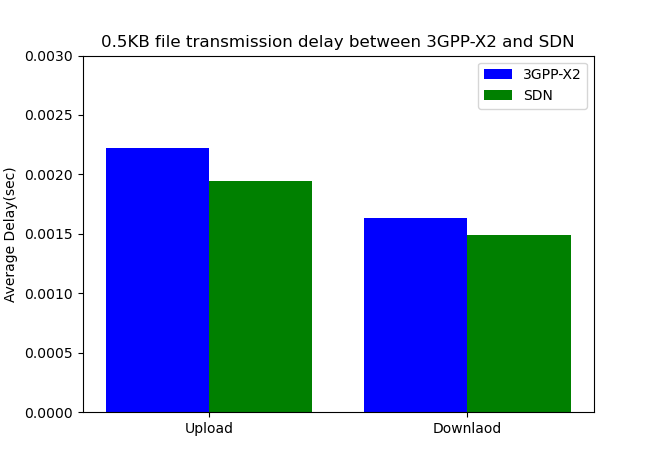
\includegraphics[width=240pt]{picture/0.5KB.png}
    \caption{Transmission delay(0.5KB) between routing technology of 3GPP-X2 and SDN}
    \label{fig:x2}
    
    \centering
    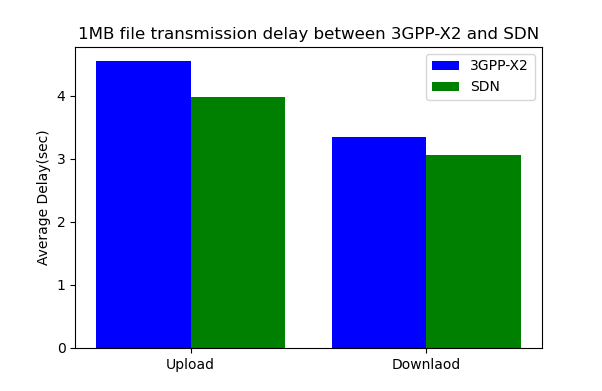
\includegraphics[width=240pt]{picture/1MB.png}
    \caption{Transmission delay(1MB) between routing technology of 3GPP-X2 and SDN}
    \label{fig:sdn}
\end{figure}

\begin{figure}
    \centering
    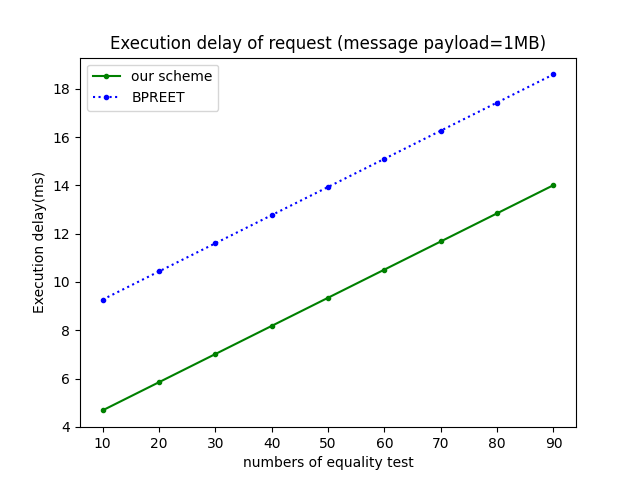
\includegraphics[width=240pt]{picture/Figure_1.png}
    \caption{Request Delay (1MB) under different number of equality test}
    \label{fig:et_1mb}
    
    \centering
    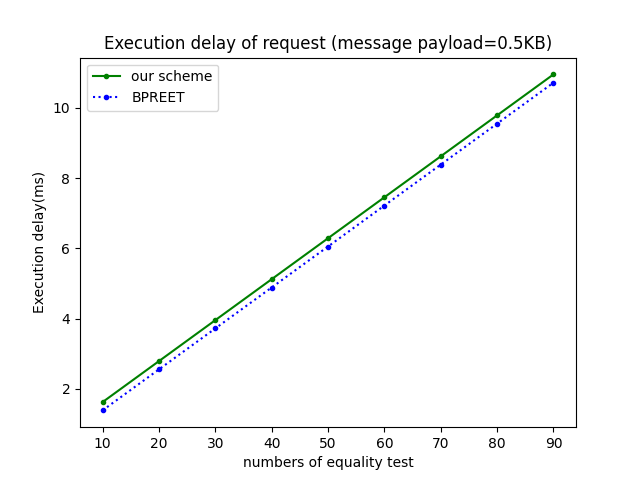
\includegraphics[width=240pt]{picture/Figure_2.png}
    \caption{Request Delay (0.5KB) under different number of equality test}
    \label{fig:et_0.5kb}
\end{figure}

\begin{table}[t!]
\caption{SIMULATION CONFIGURATIONS}
\label{tab:setting}
\centering
\begin{tabular}{ |p{4cm}|p{4cm}|  }
 \hline
 \multicolumn{2}{|c|}{Network Topology} \\
 \hline
 simulation area & 1000 m x 1000 m \\
 \hline
 Numbers of gNBs & 53 \\
 \hline
 Position of the gNB & manually set every 200 meters \\
 \hline
 Number of the UE & 100 \\
 \hline
 \multicolumn{2}{|c|}{UE Mobility} \\
 \hline
 Trace Generation & OpenStreetMap \\
 \hline
 UE speed & 0 $\sim$ 80 km/hr \\
 \hline
 \multicolumn{2}{|c|}{NS3 Configuration} \\
 \hline
 gNB Transmission Power & 23 (dbm) \cite{5GNR} \\
 \hline
 UE Transmission Power & 10 (dbm) \\
 \hline
 Transport Layer protocol & UDP protocol \\
 \hline
 Path Loss Model & Friis Propagation Loss Model \\
 \hline
 \multicolumn{2}{|c|}{Propagation delays} \\
 \hline
 Speed of light in wireless and wired links & 300000 km/s \\
 \hline
\end{tabular}
\end{table}

\begin{figure}[h]
    \centering
    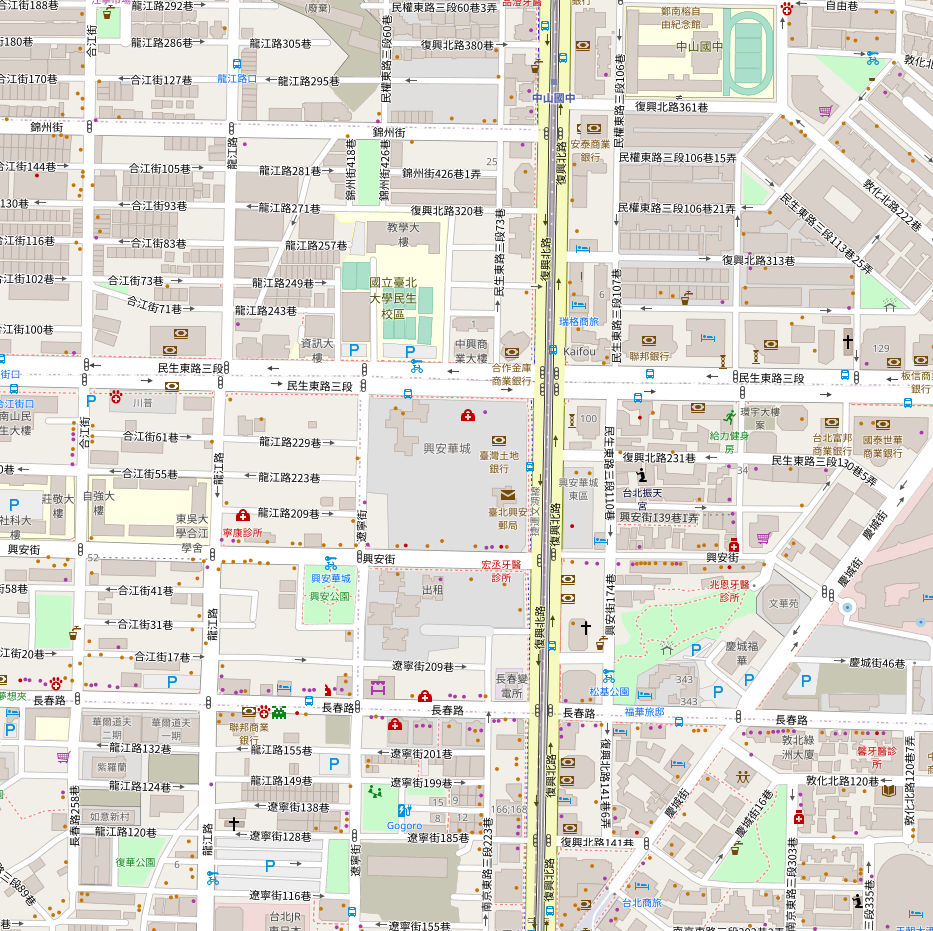
\includegraphics[width=240pt]{picture/7.png}
    \caption{The range of map selected by OpenStreetMap}
    \label{fig:OpenStreetMap}
\end{figure}

In respect of ns-3, we developed a simulator of the X2-based LTE handover procedure with and without SDN (see Fig. \ref{fig:architecture}) in order to compare the latency improvement between SDN and traditional LTE handover procedure (3GPP-X2 handover). We implemented the message uploading, downloading, and message exchange and processing of the different network nodes. Furthermore, we also simulated the transmission and propagation delays for each link (see TABLE \ref{tab:setting}). We verified that the handover procedure works correctly. Furthermore, we measured the transmission delay of uplink and downlink between UE and the remote server. Also, we compared the transmission delay between the SDN-enabled procedure and the traditional LTE X2-based handover procedure. The result is shown in Fig \ref{fig:x2} and Fig \ref{fig:sdn}. With SDN, the latency in the BPSDQS is less than that in the BPREET, around 8\%$\sim$12\%. For example, to upload a 1MB message (as video transmission) from a UE to remote server (IPFS and blockchain oracle), BPSDQS only takes 3973.65ms while BPREET needs 4545.35ms. To download a 1MB message from the remote server to the UE, BPSDQS only takes 3058.92ms while BPREET needs 3340.35ms. To upload a 0.5KB message (as request query) from a UE to the remote server, BPSDQS only takes 1.94ms while BPREET needs 2.21ms. To download a 0.5KB message from the remote server to the UE, BPSDQS only takes 1.49ms while BPREET needs 1.63ms. In Fig. \ref{fig:et_1mb} , we can see that our scheme is much faster than BPREET if data user request for a message which has a large payload such as video record. On the other hand, Fig. \ref{fig:et_0.5kb} shows that when the message payload is small, BPSDQS and BPREET yield competitive delay.


\subsection{Computation Cost Analysis}
% 演算法的計算複雜度
  The ecliptic curve in our experiment is an asymmetric elliptic curve called alt\_bn128(also called BN254 or BN256) with a 100-bit security level. Elliptic curve E: $y^2 = x^3 + 3$ mod $p$, where $p$ is 254-bit prime number. Some notations about the execution time of each operation are shown in TABLE \ref{tab:execution_time} \cite{BPREET}. Let $T_{g1}, T_{g2}, T_{gT}$ denote the scalar multiplication operations in groups $G_1, G_2, G_T$, respectively. Let $T_e$ denotes the bilinear pairing operation: ${e:G_1\times G_2 \to G_T}$. $T_{H_1}$, $T_{H_2}$ denote two hash-to-point operations on $H_1: \{0,1\}^{*} \to G_1$ and $H_2: \{0,1\}^{*} \to G_2$, respectively. And $T_{xor}$ denotes an xor operation whose computational complexity is usually negligible. 
  
\begin{table*}[t!]
\centering 
\caption{EXECUTION TIME OF DIFFERENT CRYPTOGRAPHIC OPERATIONS \cite{BPREET}}
\begin{tabular}{|c|p{25em}|c|}
    \hline
        Notations & Descriptions & Execution time(millisecond) \\
    \hline
        $T_{g1}$ & The scale multiplication on $G_1$ based on bilinear pairing & 9.56 \\
    \hline
        $T_{g2}$ & The scale multiplication on $G_2$ based on bilinear pairing & 21.56 \\
    \hline
        $T_{gT}$ & The scale multiplication on $G_T$ based on bilinear pairing & 48.81 \\
    \hline
        $T_e$ & bilinear pairing operation & 116.62 \\
    \hline
        $T_{H1}$ & hash-to-point operation: $\{0,1\}^* \to G_1$ & 2.07 \\
    \hline
        $T_{H2}$ & hash-to-point operation: $\{0,1\}^* \to G_2$ & 14.32 \\
    \hline
        $T_{aes}$ & aes-128-cbc symmetric key en/decryption & 6.63 \\
    \hline
\end{tabular}
\label{tab:execution_time}
\end{table*}
  
  TABLE \ref{tab:complexity} 
  summarizes the computational complexity of each cryptographic phase. In TABLE \ref{tab:request_overhead}, the analysis is divided into two parts; the first part analyzes the computational complexity when a data owner publishes traffic information in the system. The second part measures the computational complexity when a data user requests traffic information in the system.
 $T_{x2-ul-0.5kb}$ and $T_{x2-ul-1mb}$ denote the delay of uploading 0.5KB and 1MB data from a UE to the remote server under 3GPP-X2 handover architecture, respectively. $T_{x2-dl-0.5kb}$ and $T_{x2-dl-1mb}$ denote the delay of uploading 0.5KB and 1MB data from the remote server to the UE under the 3GPP-X2 handover architecture, respectively. $T_{sdn-ul-0.5kb}, T_{sdn-ul-1mb}$ denote the delay of uploading 0.5KB and 1MB data from the UE to the remote server under SDN-enabled architecture. $T_{sdn-dl-0.5kb}$ and $T_{sdn-dl-1mb}$ denote the delay of download 0.5KB and 1MB data from remote server to the UE under SDN-enabled handover architecture, respectively. Note that variable $n$ in TABLE \ref{tab:request_overhead} indicates the number of times that the algorithm Test needs to be executed by the corresponding scheme.
 %Note that $n$ in TABLE \ref{tab:request_overhead} indicates the times the algorithm $Test$ needs to be executed by the corresponding scheme. 
 As we can see in TABLE \ref{tab:request_overhead}, BPSDQS has higher overhead against BPREET in terms of computational complexity; we consider this can be seen as a trade-off for sustainable data accessibility. Fortunately, the overall response delay of our BPSDQS outperforms that of BPREET thanks to the slight extra computational cost.

\begin{table}[t!]
\centering 
\caption{COMPUTATIONAL COMPLEXITY}
\begin{tabular}{|p{2cm}|p{2cm}|p{2cm}|}
    \hline
    Phase & BPREET & BPSDQS \\
    \hline
    $Encrypt_{asym}$ & $4T_{g1}+T_{g2}$ & $4T_{g1}+T_{g2}$ \\
    \hline
    $Decrypt_{asym}$ & $T_{g1}$ & $T_{g1}$ \\
    \hline
    $ReKey$ & $2T_{g1}$ & $2T_{g1}$ \\
    \hline
    $Trapdoor$ & $3T_{g1}$ & $3T_{g1}$ \\
    \hline
    $Test$ & $T_{e}$ & $T_{e}$ \\
    \hline
    $ReEncrypt$ & $T_{xor}$ & $T_{xor}$ \\
    \hline
    $ReDecrypt$ & $3T_{g1}+2T_{g2}$ & $3T_{g1}+2T_{g2}$ \\
    \hline
    $En/Decrypt_{sym}$ & - & $T_{aes}$ \\
    \hline
\end{tabular}
\label{tab:complexity}
\end{table}

\begin{table*}[t!]
\centering 
\caption{CALCULATION OVERHEAD FOR PUBLISHING AND INFORMATION ACCESS }
\begin{tabular}{|c|p{7cm}|p{9cm}|}
    \hline
    Scheme & Publishing & Data Request \\
    \hline
    BPREET \cite{BPREET} & $T_{x2-ul-0.5kb}$ + $Encrypt_{asym}$ + $Encrypt_{sym}$ & $T_{x2-ul-0.5kb}$ + $T_{x2-ul-1mb}$ + $T_{x2-dl-1mb}$ + $Encrypt_{asym}$ + $(n)Test$ + $2Trapdoor$ + $ReKey$ + $ReEncrypt$ + $ReDecrypt$ + $Decrypt_{sym}$  \\
    \hline
    BPSDQS & $MAX(T_{sdn-ul-1mb}, T_{sdn-ul-0.5kb})$ + $Encrypt_{asym}$ + $Encrypt_{sym}$ & $3T_{sdn-ul-0.5kb}$ + $2T_{sdn-dl-0.5kb}$ + $T_{sdn-dl-1mb}$ + $Encrypt_{asym}$ + $(n+2)Test$ + $2Trapdoor$ + $ReKey$ + $ReEncrypt$ + $ReDecrypt$ + $Decrypt_{sym}$  \\
    \hline
\end{tabular}
\label{tab:request_overhead}
\end{table*}

\begin{table*}[t!]
\centering
\caption{COMPARATIVE SUMMARY - FEATURES}
\label{tab:Comparative_summary}
\begin{tabular}{|c|p{2.5cm}|p{2.5cm}|p{2.5cm}|p{2.5cm}|p{2.5cm}|}
    \hline
        Scheme & Decentralization \& Transparency & Confidentiality \& Searchability & Sustainable Data Accessibility & Supporting Large Amount Data Transmission & Supporting Large Amount Data Storage \\
    \hline
        BECADT \cite{BECADT} & \checkmark & x & x & x & x \\
    \hline
        BST \cite{BST} & \checkmark & x & x & \checkmark & x \\
    \hline
        BPREET \cite{BPREET} & \checkmark & \checkmark & x & x & x \\
    \hline
        ABAKA \cite{ABAKA} & x & x & x & \checkmark & \checkmark \\
    \hline
        BPSDQS & \checkmark & \checkmark & \checkmark & \checkmark & \checkmark \\
    \hline
\end{tabular}
\end{table*}

\subsection{ON-OFF Model}
To model the online and offline status change of a UE, we introduce a two-state Markov chain, known as the ON/OFF model, which is depicted in Fig. \ref{fig:onoff}. The ON/OFF model captures the fact that a data owner will not always be connected to the system. Instead, she may connect to the system for a certain period of time (the ON state) and then go offline for a while (the OFF state). She repeats the on-off behavior continuously. With the ON/OFF model, we assume that the time that the data owner stays online or offline is exponentially distributed with parameters $\lambda$ and $\mu$, respectively. That is, the average time that the data owner stays online or offline is $1/\lambda$ and $1/\mu$, respectively.
%Assume that a data owner's car will not always be connected to the Internet. After being connected to the Internet for a period of time, the data owner may go offline for a period of time, and show up online again. These behaviors will repeat. Assume that the rate of a data owner to connect to the Internet and the rate of a data owner to be off-line are both exponential distributed with parameters $\lambda$ and $\mu$ (that is, the average time of online and offline is $1⁄\lambda$ and $1⁄\mu$). 

According to the on-off model, the probability that a data owner will be online is $\frac{\mu}{\lambda+\mu}$, and the probability that she will be offline is $\frac{\lambda}{\lambda+\mu}$. We assume the delay to obtain the data is $d$ when a data owner is online. Considering the status of the data owner, the average response delay when a data user send a request to the BPSDQS system is given by:

\begin{equation}
    \frac{\mu}{\lambda+\mu}*d + \frac{\lambda}{\lambda+\mu}*(\frac{1}{\mu}+d),
\end{equation}

where an additional delay $1/\mu$ is the waiting delay for the data owner to go online. In our experiments, 
the average online time $\frac{1}{\lambda}$ varies from 10 to 50 minutes, while the average offline time $\frac{1}{\mu}$ varies from 1 to 2 times of the online time. In Fig. \ref{fig:delay_onoff}, we compare the response delay between our scheme and BPREET. The ratio of the average online time to the average offline time in the figure is set to $1, 2/3, 1/2$, respectively. When the ratio of the average online time to the average offline time is set to $1$, and the online time is over 10 minutes, the average delay of the request-response time in our scheme can saving over $98.8\%$. When the ratio of the average online time to the average offline time is set to $2/3$, and the online time is over 10 minutes, the average delay of the request-response time in our scheme can saving over $99.3\%$. When the ratio of the average online time to the average offline time is set to $1/2$, and the online time is over 10 minutes, the average delay of the request-response time in our scheme can saving over $99.5\%$. In our scheme, no matter whether the data owner is online or offline when the data user sends out her request, she can get the response in a much shorter delay.

\begin{figure}[h]
    \centering
    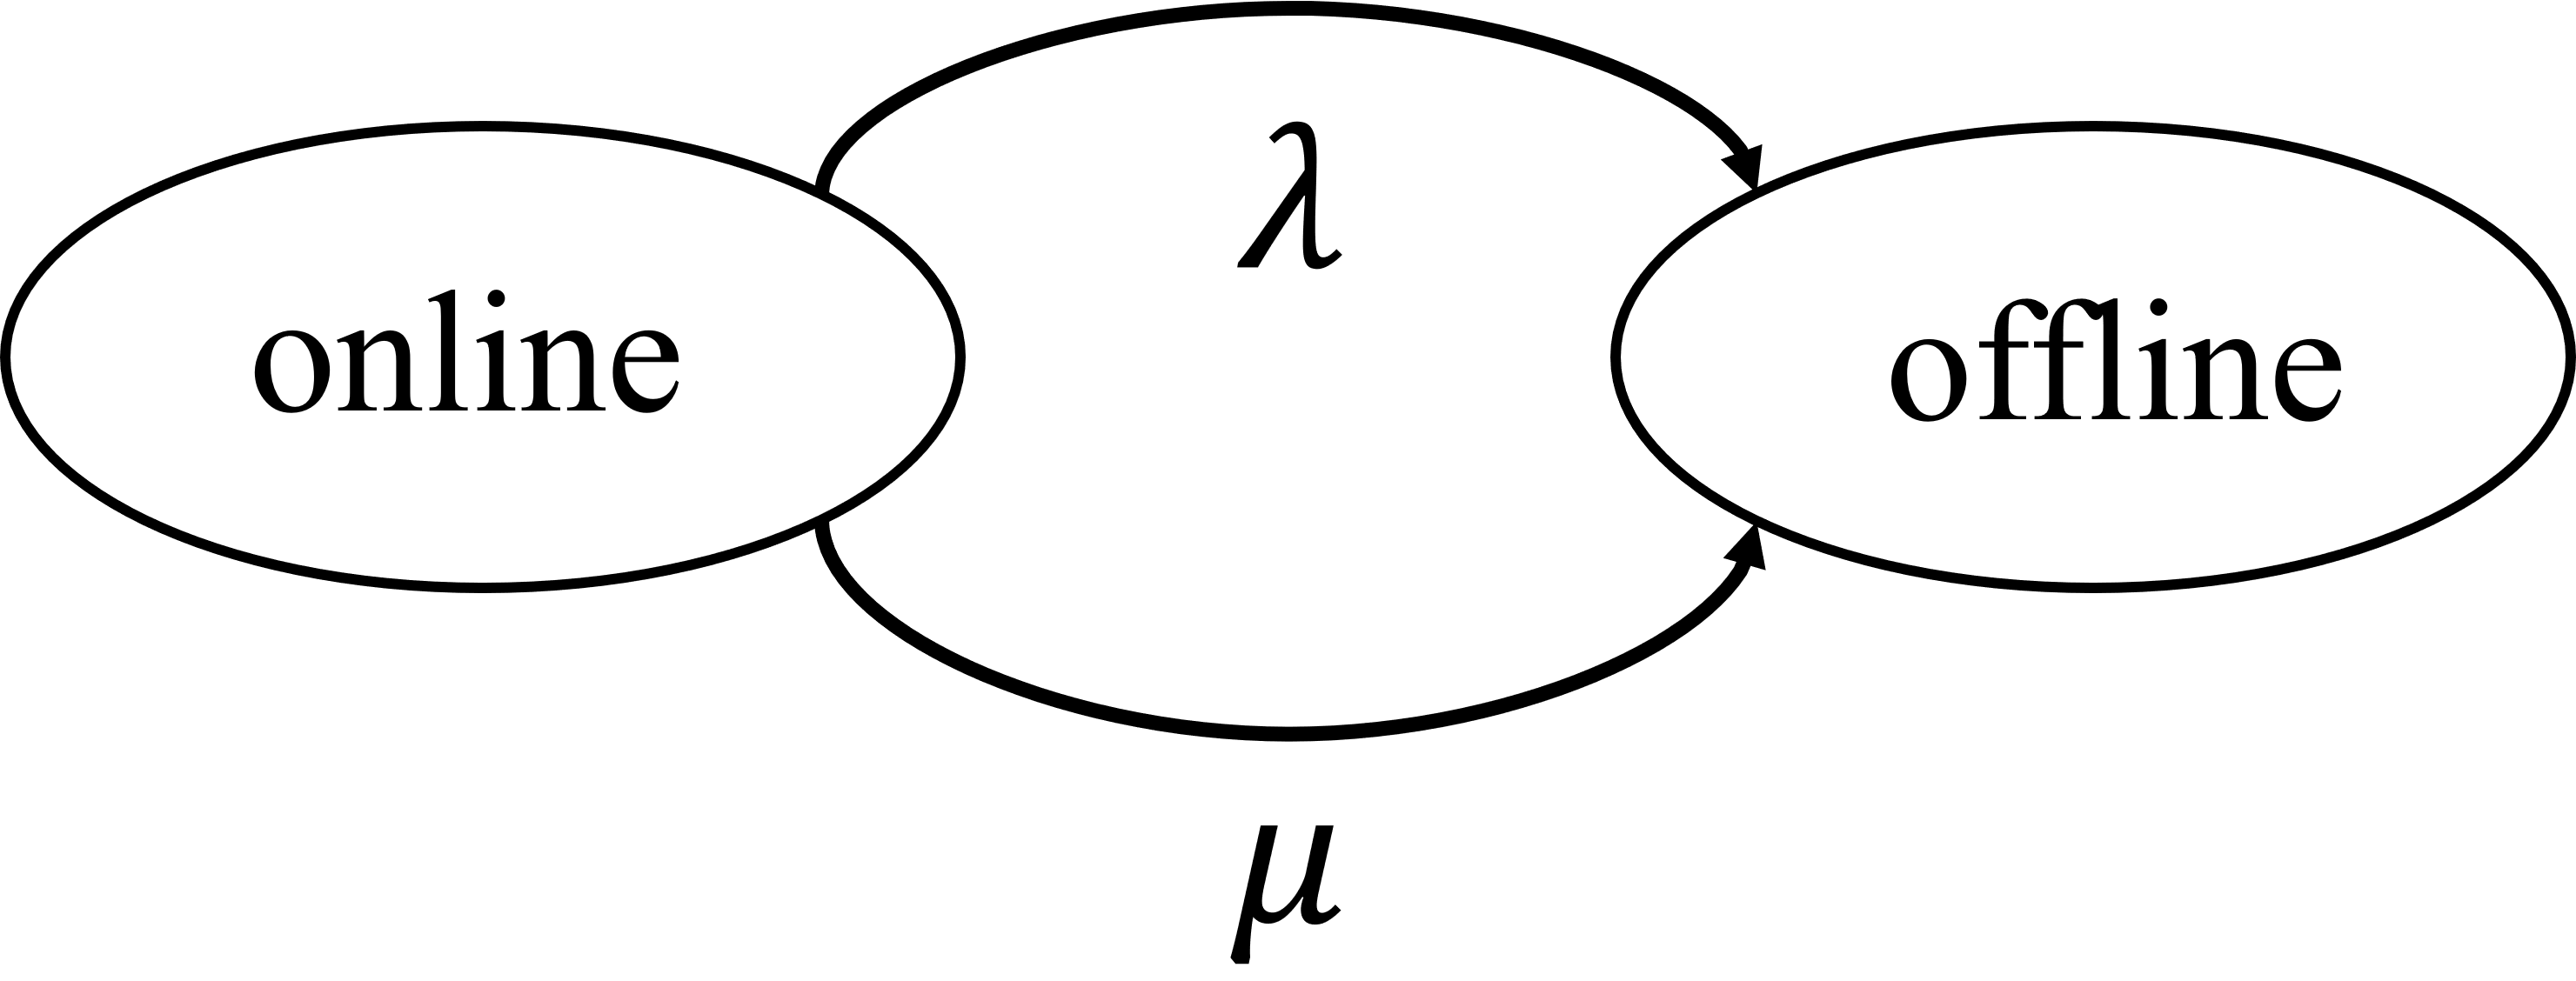
\includegraphics[width=180pt]{picture/onoff3.png}
    \caption{ON-OFF Model}
    \label{fig:onoff}
\end{figure}

\begin{figure}[h]
    \centering
    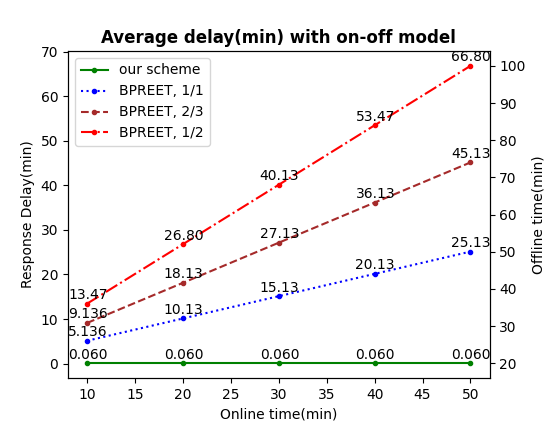
\includegraphics[width=260pt]{picture/onoff_plot3.png}
    \caption{Average delay with on-off model, the ratio of the average online time to the average offline time in BPREET is $1$, $2/3$, and $1/2$.}
    \label{fig:delay_onoff}
    
    \centering
    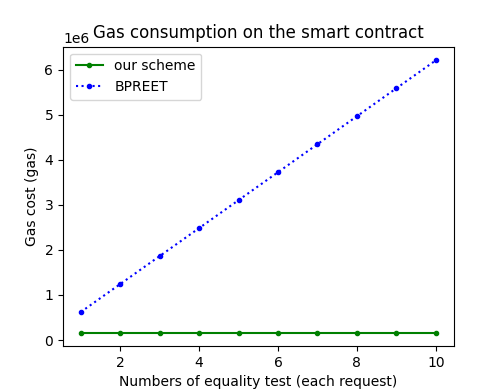
\includegraphics[width=260pt]{picture/gas2.png}
    \caption{Comparison of Gas consumption}
    \label{fig:gas_cost}
\end{figure}

\subsection{Gas consumption}
In the following experiment, we compare the gas consumption of the proposed scheme with that of BPREET. To compare the gas consumption of each scheme, we deploy the smart contract and measure the execution cost on the Ethereum Remix IDE. In Fig. \ref{fig:gas_cost}, we compare the gas consumption between our scheme and BPREET. As we can observe from Fig. \ref{fig:gas_cost}, our scheme consumes much less gas than BPREET. The rationale is that the major gas consumption of the smart contract is performing the equality test. In our proposed scheme, with the help of oracle, our scheme only performs the equality test once, while the BPREET needs to perform the equality test many times in order to match the keywords. 
%In comparison with the gas consumption, we deploy the smart contract and measure the execution cost on the Ethereum Remix IDE. As shown in Fig. \ref{fig:gas_cost}, we compare the gas cost between our scheme and BPREET. In our scheme, we only have to do the equality test one time although the BPREET needs to do the equality test many times in order to match for the keyword. In our scheme, oracle helped to carry out the operations of equality test, which can saving the gas cost in each request.

\subsection{Comparative Summary}
 In the comparative summary, we focus on five key features, including transparency, confidentiality \& searchability, sustainable data accessibility, supporting large amount data transmission, and supporting large amount data storage.
 
\subsubsection{Decentralization \& Transparency}
Decentralization requires that the whole scheme does not rely on a central server. For example, in VANETs, a single server may not be able to afford the traffic message generated from tons of vehicles. Therefore, the decentralization feature can avoid the single-point failure vulnerability. On the other hand, transparency means that
other users can easily examine the exchange records and computational results. In general, a centralized system usually cannot provide transparency, which may jeopardize the credibility of the system. 


\subsubsection{Confidentiality \& Searchability}
Confidentiality \& searchability requires that a data user can search data in the system without exposing the privacy information of the data owner.
  
\subsubsection{Sustainable Data Accessibility}
Stable data accessibility represents that the data query service should always be accessible by a data user.
  
\subsubsection{Supporting Large Amount Data Transmission}
A system architecture can afford a large amount of data transmission, such as video transmission.
  
\subsubsection{Supporting Large Amount Data Storage}
A system architecture can store a large amount of data in the system. Since the size of a block in the blockchain is limited, there should be another way to store large amounts data, such as video records of traffic information.

Table \ref{tab:Comparative_summary} shows the comparison results. The entry \checkmark shows that the scheme meets the demand, and the entry x indicates that the scheme does not meet the requirement. And it is noted that among all the schemes compared in Table \ref{tab:Comparative_summary}, only our scheme meets all the features. 

% 應該要先寫 SUMO 的參數跟 NS3 的參數?

\section{CONCLUSION AND FUTURE WORK}
In this paper, a fair and privacy-preserving data query system for VANETs has been proposed. The proposed scheme provides features of sustainable data accessibility and a large amount of data storage. Based on blockchain technology, the proposed scheme does not rely on a central server. With the immutability and accountability features of blockchain, we also provide the incentive mechanism to encourage users to share their traffic information like video records. In order to improve the data transmission efficiency of the system, we introduce SDN into our system architecture. Our simulation results confirm that SDN can reduce the data transmission latency between the UE and the remote server. The experiment results show that our scheme provides much more stable data accessibility and efficiency. A comparative summary demonstrated that our scheme is a decent scheme for VANETs in the real world. As for future work, we will consider about the design of independent proxy agents by the advanced cryptography and smart contracts, and the verification of SDN predictive route path on blockchain to fit the requirements of VANETs in the real world.


% \appendices
% \section{Proof of the ...}
% Appendix one text goes here.


% \section{}
% Appendix two text goes here.

% \section*{Acknowledgment}


% The authors would like to thank...



\ifCLASSOPTIONcaptionsoff
  \newpage
\fi


\begin{thebibliography}{1}
% You can use other form of bib file by changing here... 

\bibitem{Survey on various mechanisms for Secure and Efficient VANET communication}
V. Vijayalakshmi, M. Sathya, S. Saranya, and C. Selvaroopini, "Survey on various mechanisms for Secure and Efficient VANET communication," IEEE International Conference on Information Communication and Embedded Systems, 2014.

\bibitem{Blockchain based intelligent vehicle data sharing framework}
M. Singh, and S. Kim, “Blockchain based intelligent vehicle data sharing framework,” CoRR, vol. abs/1708.09721, 2017.

\bibitem{Security Issues inVehicular Ad-hoc Network(VANET)}
R. Kaur, T. P. Singh, V. Khajuria, "Security Issues inVehicular Ad-hoc Network(VANET)," International Conference on Trends in Electronics and Informatics (ICOEI), pp. 884-889, May 2018.

\bibitem{Securing vehicular ad hoc networks}
M. Raya, and J.-P. Hubaux, “Securing vehicular ad hoc networks,” J. Comput. Secur., vol. 15, no. 1, pp. 39–68, 2007.

\bibitem{Blockchain technology on the way of autonomous vehicles development}
S. Narbayeva, T. Bakibayev, K. Abeshev, I. Makarova, K. Shubenkova, and A. Pashkevich, “Blockchain technology on the way of autonomous vehicles development,” Transportation Research Procedia, vol. 44, pp. 168–175, Jan. 2020.

\bibitem{A survey on the security of blockchain systems}
 X. Li, P. Jiang, T. Chen, X. Luo, and Q. Wen, “A survey on the security of blockchain systems,” Future Generation Computer System, vol. 2017, pp. 1–13, August 2017.

\bibitem{A blockchain construct for energy trading against sybil attacks}
U. Asfia, V. Kamuni, S. Sutavani, A. Sheikh, S. Wagh, and N. M. Singh, “A blockchain construct for energy trading against sybil attacks,” Mediterranean Conference on Control and Automation (MED), pp. 422–427, July 2019.

\bibitem{Regional blockchain for vehicular networks to prevent 51 attacks}
R. Shrestha and S. Y. Nam, “Regional blockchain for vehicular networks to prevent 51\% attacks,” IEEE Access, vol. 7, pp. 95 033–95 045, 2019.

\bibitem{BECADT}
H. Liu, P. Zhang, G. Pu, T. Yang, S. Maharjan and Y. Zhang, "Blockchain empowered cooperative authentication with data traceability in vehicular edge computing," IEEE Transactions on Vehicular Technology, pp. 1-1, April 2020.

\bibitem{BST}
L. Xie, Y. Ding, H. Yang and X. Wang, "Blockchain-based secure and trustworthy Internet of Things in SDN-enabled 5G-VANETs," IEEE Access, vol. 7, pp. 56656-56666, April 2019.

\bibitem{Secure blockchain-based communication scheme for connected vehicles}
J. A. Leon Calvo, and R. Mathar, “Secure blockchain-based communication scheme for connected vehicles,” European Conference on Networks and Communications (EuCNC), pp. 347–351, June 2018.

\bibitem{Creditcoin: A privacy-preserving blockchain-based incentive announcement network for communications of smart vehicles}
L. Li, J. Liu, L. Cheng, S. Qiu, W. Wang, X. Zhang, and Z. Zhang, “Creditcoin: A privacy-preserving blockchain-based incentive announcement network for communications of smart vehicles,” IEEE Transactions on Intelligent Transportation Systems, vol. 19, no. 7, pp. 2204–2220, 2018.

\bibitem{Speedychain: A framework for decoupling data from blockchain for smart cities}
R. A. Michelin, A. Dorri, M. Steger, R. C. Lunardi, S. S. Kanhere, R. Jurdak, and A. F. Zorzo, “SpeedyChain: A Framework for Decoupling Data from Blockchain for Smart Cities,” in Proceedings of the 15th EAI International Conference on Mobile and Ubiquitous Systems: Computing, Networking and Services, MobiQuitous ’18, (New York, NY, USA), pp. 145–154, 2018.

\bibitem{BPREET}
B. Chen, D. He, N. Kumar, H. Wang and K. R. Choo, "A Blockchain-Based Proxy Re-Encryption with Equality Test for Vehicular Communication Systems,"  IEEE Transactions on Network Science and Engineering, pp.1-1, June 2020.

\bibitem{Blockchain-enabled security in electric vehicles cloud and edge computing}
H. Liu, Y. Zhan, and T. Yang, ”Blockchain-enabled security in electric vehicles cloud and edge computing,” IEEE Network, vol. 32, no. 3, pp.78- 83, June 2018.

\bibitem{Introduction to Modern Cryptography}
J. Katz and Y. Lindell, Introduction to Modern Cryptography (Chapman $\&$ Hall/CRC Cryptography and Network Security Series). London, U.K.: Chapman & Hall, 2007.

\bibitem{New directions in cryptography}
W. Diffie, and M. Hellman, “New directions in cryptography,” IEEE Transactions on Information Theory, vol. 22, no. 6, pp. 644–654, Nov. 1976.

\bibitem{ABAKA}
Jiun-Long Huang, Lo-Yao Yeh, and Hung-Yu Chien, "ABAKA: An Anonymous Batch Authenticated and Key Agreement Scheme for Value-Added Services in Vehicular Ad Hoc Networks", IEEE Transactions on Vehicular Technology, vol. 60, no. 1, pp. 248–262, Jan. 2011.

\bibitem{Proxy re-encryption with keyword search}
J. Shao, Z. Cao, X. Liang, and H. Lin, “Proxy re-encryption with keyword search,” Information Sciences, vol. 180, no. 13, pp. 2576–2587, 2010.

\bibitem{Blockchain for secure and efficient data sharing in vehicular edge computing and networks}
J. Kang, R. Yu, X. Huang, M. Wu, S. Maharjan, S. Xie, and Y. Zhang, ”Blockchain for secure and efficient data sharing in vehicular edge computing and networks,” IEEE Internet Things J., vol. 6, no. 3, pp.4660-4670, June 2019.

\bibitem{sumo}
P. A. Lopez et al., "Microscopic Traffic Simulation using SUMO," in 2018 21st International Conference on Intelligent Transportation Systems (ITSC), Maui, HI, pp. 2575-2582, doi: 10.1109/ITSC.2018.8569938, 2018.

\bibitem{ns3}
G. F. Riley, and T. R. Henderson, “The ns-3 network simulator,” in Modeling and Tools for Network Simulation. Springer, pp. 15–34, 2010.

\bibitem{5GNR}
3GPP TS 38.104 v15.5.0; Base Station (BS) radio transmission and reception, (Release 15), May 2019.

% \bibitem{Blockchain-based software-defined industrial Internet of Things: A dueling deep Q-learning approach}
% C. Qiu, F. R. Yu, H. Yao, C. Jiang, F. Xu and C. Zhao, "Blockchain-based software-defined industrial Internet of Things: A dueling deep Q-learning approach", IEEE Internet of Things Journal, pp. 4627 – 4639, June, 2019.

% \bibitem{Toward Blockchain-Based Fair and Anonymous Ad Dissemination in Vehicular Networks}
% M. Li, J. Weng, A. Yang, J. Liu and X. Lin, "Toward Blockchain-Based Fair and Anonymous Ad Dissemination in Vehicular Networks," IEEE Transactions on Vehicular Technology, pp. 11248 – 11259, September, 2019

% \bibitem{Bars: a blockchain-based anonymous reputation system for trust management in vanets}
% Z. Lu, Q. Wang, G. Qu, and Z. Liu, “Bars: a blockchain-based anonymous reputation system for trust management in vanets,” in 2018 17th IEEE International Conference On Trust, Security And Privacy In Computing And Communications/12th IEEE International Conference On Big Data Science And Engineering (TrustCom/BigDataSE), pp. 98–
% 103, IEEE, 2018.

% \bibitem{IEEEhowto:kopka}
% M. Singh and S. Kim, “Branch based blockchain technology in intelligent vehicle,” Comput. Networks, vol. 145, pp. 219–231, 2018.

% \bibitem{IEEEhowto:kopka}
% S. Gong, E. Tcydenova, J. Jo, Y. Lee, and J. Park, “Blockchain-based secure device management framework for an internet of things network in a smart city,” Sustainability, vol. 11, p. 3889, 07 2019.

% \bibitem{IEEEhowto:kopka}
% A. Ranchal-Pedrosa and G. Pau, “Chargeltup: On blockchain-based technologies for autonomous vehicles,” in Proceedings of the 1st Workshop on Cryptocurrencies and Blockchains for Distributed Systems, pp. 87–92, 06 2018.

% \bibitem{IEEEhowto:kopka}
% “Steps you can take to correct a mistake in the police report after your car accident,” in braunslaw.com, 2019.

% \bibitem{IEEEhowto:kopka}
% R. Huckstep, “Four ways autonomous vehicles will change auto insurance,” in the-digital-insurer.com, 2018.

% \bibitem{IEEEhowto:kopka}
% D. Carlson, “The autonomous vehicle revolution: How insurance must adapt,” in marsh.com, 2018.

% \bibitem{IEEEhowto:kopka}
% D. Barnett, “Autonomous cars and auto insurance: What’s going to happen,” in atlantainsurance.com, 2018.

% \bibitem{IEEEhowto:kopka}
% H. Guo, E. Meamari, and C.-C. Shen, “Blockchain-inspired event recording system for autonomous vehicles,” in 2018 1st IEEE International Conference on Hot Information-Centric Networking (HotICN), pp. 218–222, 2018.

% \bibitem{IEEEhowto:kopka}
% T. Aste, P. Tasca, and T. Di Matteo, “Blockchain technologies: The foreseeable impact on society and industry,” Computer, vol. 50, pp. 18–28, 01 2017.

% \bibitem{IEEEhowto:kopka}
% M. Cebe, E. Erdin, K. Akkaya, H. Aksu, and S. Uluagac, “Block4forensic: An integrated lightweight blockchain framework for forensics applications of connected vehicles,” arXiv preprint arXiv:1802.00561, 2018.

\end{thebibliography}



% \begin{IEEEbiography}{Nong-Xiang Shen}
% Biography text here.
% \end{IEEEbiography}

%It is not necessary to upload the biography when you submit your manuscript.


\end{document}


